\documentclass[a4paper]{article}

\usepackage{microtype}
\usepackage{fullpage}
\usepackage{mathtools}
\usepackage{amsfonts}
\usepackage{tikz}
\usepackage{pgfplots}
\usepackage{pgfplotstable}
\usepackage{hyperref}
\usepackage[noabbrev,nameinlink]{cleveref}
\usepackage{amsthm}
\usepackage{xcolor}
\usepackage{caption}
\usepackage{subcaption}
\usepackage{setspace}
\usepackage[backend=biber,style=authoryear,maxbibnames=99,hyperref=true]{biblatex} 

\setstretch{1.15}

\addbibresource{src/paper/references.bib}

\usepgfplotslibrary{fillbetween}
\usetikzlibrary{shapes}
\usetikzlibrary{intersections}
\pgfplotsset{compat=1.17}

\newtheorem{definition}{Definition}
\newtheorem{observation}{Observation}
\newtheorem{proposition}{Proposition}
\newtheorem{corollary}{Corollary}
\newtheorem{lemma}{Lemma}
\newtheorem{assumption}{Assumption}

\crefname{assumption}{assumption}{assumptions}
\Crefname{assumption}{Assumption}{Assumptions}
\crefname{observation}{observation}{observations}
\Crefname{observation}{Observation}{Observations}

\newcommand{\dt}{\mathrm{d}t}
\newcommand{\ds}{\mathrm{d}s}
\newcommand{\di}{\mathrm{d}i}
\newcommand{\E}{\mathbb{E}}

\definecolor{myblue}{rgb}{0.3, 0.45, 0.69}
\definecolor{myred}{rgb}{0.87, 0.52, 0.32}
\definecolor{mygreen}{rgb}{0.34, 0.68, 0.45}

\pgfplotstableread[col sep=comma]{out/figures/equilibrium_profit_onesided_scale-1_lambda-1.csv}\equilibrium
\pgfplotstableread[col sep=comma]{out/figures/equilibrium_welfare_onesided_scale-0.6_lambda-1.csv}\equilibriumFullSurplusOneSided
\pgfplotstableread[col sep=comma]{out/figures/equilibrium_welfare_twosided_scale-0.6_lambda-1.csv}\equilibriumFullSurplusTwoSided
\pgfplotstableread[col sep=comma]{out/figures/equilibrium_profit_onesided_scale-1_lambda-0.5.csv}\equilibriumProfitOneSidedLowLambda

\title{Hybrid platforms and bargaining power}
\author{Martin Stancsics}

\begin{document}

\maketitle

\begin{abstract}
    This paper explores the effects of a platform selling their own products in addition to acting as intermediaries (hybrid platforms) in a setting when bargaining takes place between the platform and the potential entrants.
    It highlights a so-far underappreciated aspect of hybrid platforms: having their own products increases their bargaining power over the other sellers.
    This change in bargaining might lead to lower entry, and thus reduced product variety which in turn can have negative welfare consequences for the consumers.
    The results and methods described in this paper are also applicable to other similar settings, such as vertical integration with a monopolistic upstream supplier.
\end{abstract}


\section{Motivation}

Even though the economics literature offers no unambiguous definition for what platforms are, there seems to be a consensus that they are of key importance for the modern economy, and are getting even more so in the future.
Although market structures resembling various aspects of what we call platforms have existed for some time, the term has only gained widespread usage in the 2000s, with the advent of digitization, and a number of behemoth technology companies playing matchmakers on the internet.
Since then, platforms have become a buzzword in the business world, the subject of increasing regulatory scrutiny, and also a topic of intense academic interest.

Platforms have a number of unique features that make them different from more traditional market structures.
The most prominent of those are multi-sidedness and network effects, which most of the early literature \parencite[for an overview, see][]{rochet2006two} and policy debate \parencite[e.g.][]{fletcher2021consumer,calvano2021market} has focused on.
However, in the more recent years, another important and potentially concerning aspect has been getting more attention: the hybrid operation of certain platforms.
Essentially, this means that platforms act as an intermediary (deciding the rules) and a market participant (competing with other entrants) at the same time.

While hybrid platforms are not a completely new phenomenon, they are becoming more and more common in various industries.
Perhaps the most prominent example is Amazon, which, on the one hand sells its own products, and at the same time hosts ax large number of third-party sellers.
However, examples abound in other industries, as well.
For example, each of the largest digital distribution platforms for computer and smartphone applications (Google Play, Apple App Store and Microsoft Store) sell their own applications besides their third party offerings.
In the video game industry, platform owners studios and publishing games under their own brand is the standard.
Many video streaming services (e.g. Netflix, Amazon Prime Video, Hulu) offer a mix of their own and licensed content.
One can also find examples of similar behavior outside the platform setting, too.
For example BMW is preparing to sell cars directly to consumers in the US, competing with its dealership network.

As deciding the rules of the game and competing in it at the same time gives rise to some obvious concerns, policymakers have been paying increasingly close attention to these platforms in the recent years.
Various pieces of legislation have been proposed to regulate, or even ban e-commerce platforms from selling their own products \parencite[][]{phartiyal_2019,reynolds_2022,eu-2022}.
Furthermore, one of the most prominent ongoing antitrust cases, Microsoft attempting to acquire the video game publisher Activision/Blizzard for a sum of 69 billion USD, is also a case of a platform becoming increasingly hybrid.
This merger would not only increase market concentration on the software side of the video game industry, but might also have further implications for the competition between Microsoft as a platform owner and the other game developers.
The deal is currently under investigation by multiple antitrust authorities, including the US Federal Trade Commission, the European Commission, and the UK Competition and Markets Authority \parencite{livni_merced_2023}.

In parallel to the increasing regulatory interest, the academic literature has also been steadily growing on the topic of hybrid platforms.
\textcite{hagiu2022should} investigate how practices, such as self-preferencing and steering can distort competition on hybrid platforms.
They argue, however, that if such behavior is regulated, the platform selling its own products can be beneficial for consumers.
In contrast to this positive result, \textcite[]{anderson2021hybrid} find that even in the absence of such behavior, allowing hybrid operation might have negative consequences due to platforms having an incentive to exclude competitors from the market.
\textcite[]{gutierrez2021welfare} shows that general conclusions are hard to draw, and welfare effects are platform and product specific.

This paper aims to contribute to this discussion by examining an important, but so far underexplored aspect of platforms: the bargaining power disparity between them and the other market participants, and how this disparity is affected by the platforms' hybrid operation.
In particular, I propose an analytically tractable framework which captures many important aspects of bargaining between one large and a continuum of small players, and apply it to the setting of a hybrid platform facing a continuum of potential entrants.
The results show that, in the presence of bargaining, hybrid operation can indeed have negative welfare consequences for consumers.
This result is particularly striking in this otherwise distortion-free\footnote{
    In the benchmark model without bargaining, the platform's hybrid operation does not affect consumer welfare.
} setting. 
The intuition is that hybrid operation increases the platform's bargaining power against the sntrant sellers.
This in turn leads to a higher entry fee, fewer entrants, then results in lower consumer surplus.
These observations constitute a so-far overlooked aspect of hybrid platforms that policymakers should be aware of.

The closest paper to this one is \textcite{anderson2021hybrid}, which utilizes a similar model and reaches similar conclusions, although through a different mechanism.
I adapt many of the main features of their model with a couple of crucial differences.
Instead of the platform setting a percentage entry fee and being able to commit to it, I assume that (1) platforms charge a lump-sum entry fee and that (2) this entry fee is the result of a negotiation process\footnote{
    The bargaining process is modeled using a solution concept from cooperative game theory, namely the Shapley-value.
    This allows for a tractable analysis while at the same time capturing many of the important features of bargaining.
    Examples of this approach in the industrial organization literature include \textcite{montez2007downstream}, as well as \textcite{hart1990property}, \textcite{levy1997individual}, \textcite{inderst2003bargaining} and \textcite{brugemann2019intra} among others.
}
between the platform and the entrants.
The second point is a novelty not only compared to \textcite{anderson2021hybrid}, but also to the existing literature on hybrid platforms.
Furthermore, in contrast to \textcite{hagiu2022should}, this model is free from any distortive behavior, such as self-preferencing or steering, and the negative results are purely driven by changes in the platform's bargaining position.

This paper is also related to various other strands of the industrial organization literature.
For one, it belongs to the research agenda on understanding platforms and their role in the economy \parencite[e.g.][]{rochet2003platform,hagiu2004optimal,armstrong2006competition,evans2011platform,lee2014competing}.
Furthermore, it is somewhat adjacent to the literature on the importance of exclusive content \parencite[e.g.][]{hagiu2011exclusivity,lee2013vertical,dou2014sell,weeds2016tv}, with the difference that instead of exclusive content giving an advantage against competing platforms, in this paper, own products provide an advantage over entrants.
More generally, many results and concepts of this paper are also applicable outside the context of (multi-sided) platforms.
Certain structures, such as vertical relationships, or even traditional retail stores share a number of features with platforms (notably, the presence of a dominant, indispensable entity), and can be modeled in much the same way.
Therefore, the methodology and results in this paper may also be of interest to researchers studying questions such as retailers having their own private labels \parencite{steiner2004nature} or vertical integration in upstream-downstream markets \parencite{hart1990vertical,aghion2006vertical}.
\textcite{de2005vertical} and \textcite{montez2007downstream}, in which bargaining between the upstream and downstream firms take the center stage, are particularly closely related.

Finally, this paper also belongs to the not too large set of models using concepts from cooperative game theory in an industrial organization setting.
Such examples include the aforementioned \textcite{montez2007downstream}, as well as \textcite{hart1990property}, \textcite{levy1997individual}, \textcite{inderst2003bargaining} and \textcite{brugemann2019intra}, among others.
In contrast to the majority of those, which focus on games with a finite number of players, I utilize an oceanic game (a continuum of small players instead of a finite number), and demonstrate that this can considerably simplify the analysis in certain cases.
Therefore, the modeling approach presented in this paper may be of use in other settings as well.

The rest of the paper is organized as follows.
In \cref{sec:model}, I introduce a general version of the model.
After that, \cref{sec:results} demonstrates results about bargaining outcomes one can derive even in this rather abstract setting.
\Cref{sec:example} concretizes the model by assuming a specific demand system, and also presents a corresponding benchmark model without bargaining.
Finally, \cref{sec:conclusion} summarizes the results and discusses possible future work.


\section{Model}
\label{sec:model}

This section introduces the model used throughout the paper.
I use the terms ``platform'' and ``fringe sellers'', and present my ideas in the context of an intermediated market, such as an online marketplace or an application store.
However, the model is quite general, and the results apply to a broader class of settings, such as vertical markets where the upstream firm can sell directly to consumers, or retail stores with their own private labels.

Assume that there are three types of players in the market: a platform $P$, a continuum of fringe sellers $F_i$ ($i \in [0, N_C$) and a continuum of consumers $C_j$ ($j \in [0, N_C$]).
The fringe firms have one product each, which they can only sell through the platform.
Without the platform, they make zero profits.
In addition to acting as an intermediary between the fringe and the consumers, the platform itself may also produce and sell a number of products directly to the consumers.
If it does, it is referred to as a hybrid platform.

The main distinguishing feature of this model is that, instead of assuming that entry fees or royalties are set by the platform and the fringe treat it as take it or leave it offers, I assume that the platform and the fringe engage in some kind of bargaining over their total profits.
The bargaining rule, as well as other details of the model, are described in the rest of this section.


\subsection{Production}

I make use of a reduced-form, but quite general approach to model production and demand.
First, I assume that all fringe firms and consumers are ex-ante identical.
This implies two things: (1) per-consumer profits are just a function of the number of fringe and platform products, and (2) the platform's and the fringe's profits are linear in the number of consumers.\footnote{
    While normally this would exclude fixed production costs, this is not the case here.
    $\Pi$ only describes profits conditional on $N_C$ and $N_F$ players entering the platform.
    Fixed costs can be incorporated into the first stage of the game, where fringe firms decide whether to enter or not.
}
Therefore, the total profits of the platform and the fringe taken together have a simple functional form $N_C f(N_P, N_F)$.\footnote{
    Based on the same reasoning, it is easy to see that total welfare has a similar form.
}
Formally, this is described by the following assumption.
\begin{assumption}
    \label{ass:identical_fringe}
    The total profits of the platform and the fringe are described by 
    \begin{align*}
        \Pi(N_P, N_F, N_C) = N_C f(N_P, N_F),
    \end{align*}
    where $f: \mathbb{R}^+_0 \times \mathbb{R}^+_0 \to \mathbb{R}^+_0$.
\end{assumption}
Here, $N_F$ is the mass of fringe sellers, $N_C$ is the mass of consumers, and $N_P$ measures the degree to which the platform sells its own products.
For example, in a setting with differentiated products and monopolistic competition, $N_F$ and $N_P$ represent the product variety of the fringe and the platform, respectively.
$N_P = 0$ corresponds to the case when the platform is a pure intermediary, and $N_F = 0$ to the case then the platform is a pure retailer.

I will assume that, in addition to being increasing in the number of consumers, total profits are also increasing in both the number of fringe firms and the platform' products.
\begin{assumption}
    \label{ass:monotone_profits}
    $f(n_P, n_F)$ is increasing in both $n_P$ and $n_F$.
\end{assumption}
Such profit functions arise in settings in which the profit reduction from increased competition is dominated by extra sales due to increased product variety.
One such example is \textcite{anderson2020aggregative}, where the demand exhibits love for variety, while consumers have access to an outside option.
Alternatively, indirect network effects, such as those in two-sided markets, can also result in such increasing profits.
Finally, if we assume that the platform can extract consumer surplus through entry fees or some similar mechanism, then this assumption will be true for any demand system in which total surplus is increasing in product variety.


\subsection{Profit sharing}

I assume that fringe firms are unable to sell their products directly to consumers.
Instead, they must sell through the platform.
For this service, the platform may charge a fee, and obtain a share of the fringe's profits.

In the benchmark model, the platform will be able to set and commit to any lump-sum entry fee it wishes to.\footnote{
    The focus of this paper is on fees paid and entry decisions made by fringe producers, but I will also consider the case when consumers also face entry fees or subsidies.
}
The main contribution of this paper is to deviate from this usual assumption, and instead consider a setting in which the platform and the fringe engage in some form of bargaining over the total profits.
To model this in a tractable way, I propose a profit division rule that is based on the Shapley value \parencite{shapley1953additive}, or, more generally, random order values \parencite{weber1988probabilistic}.
This way of modelling bargaining outcomes has many precedents in the industrial organization literature \parencite[e.g.][]{montez2007downstream,hart1990property,levy1997individual,inderst2003bargaining,brugemann2019intra}.
In the main text, I simply propose a formula for the profit shares without going into the details of the underlying cooperative game.
The interested reader can find a more detailed discussion of how it relates to random order values in \cref{sec:cooperative_game}.

\begin{assumption}
    \label{ass:profit_sharing}
    Let $N_P, N_F, N_C \geq 0$ be the number of platform products, fringe firms and consumers, respectively.
    Thus, the value that players create together is given by $\Pi(N_P, N_F, N_C) = N_C f(N_P, N_F)$.
    Let us denote the platform's and the fringe's profit shares by $\pi_P(N_P, N_F, N_C)$ and $\pi_F(N_P, N_F, N_C)$, respectively.
    Then, the following holds:
    \begin{align*}
        \pi_P(N_P, N_F, N_C) &= N_C \int_0^1 w_P(s) f(N_P, s N_F) \ds, \\
        \pi_F(N_P, N_F, N_C) &= N_C \int_0^1 w_F(s) N_F \partial_2 f(N_P, s N_F) \ds.
    \end{align*}
    Furthermore, $w_P \geq 0$ and $w_F \geq 0$ are such that $\pi_P(N_P, N_F, N_C) + \pi_F(N_P, N_F, N_C) \leq \Pi(N_P, N_F, N_C)$.
\end{assumption}

Although the reason behind choosing this particular form for profit shares is discussed in detail in the appendix, let me highlight some important observations.
First, player's profit shares are closely related to their (weighted average) marginal contributions to the total value.
In the case of the platform, its contribution is the total value, as it is indispensable, while the fringe firms' contribution is captured by the partial derivative of the total value with respect to the number of fringe firms.
Second, the platform and the fringe do not necessarily get the entire value they create.
This is due to the fact that I also want to allow for the possibility of consumers participating in the bargaining process and getting a share of the profits, too
Finally, the profit shares depend on two types of factors: the production function $f$ and $w_P$ and $w_F$, which I will call bargaining weights.
The former is determined by the technology and demand structure, while the latter can be thought of as some king of intrinsic bargaining power.

In the later sections, I will consider specific examples for $f$ and $w_P$ and $w_F$, motivated by a Logit-like demand system, and (weighted) Shapley values, respectively.
However, for a number of results, this level of detail is not necessary, and these quite general assumptions are sufficient.

As mentioned before, one main justification for this profit allocation rule its intuitive behavior in terms of comparative statistics.
To illustrate this, let us examine what happens when one varies the substitutability between the fringe firms.
As it turns out, the platform's share increases if the fringe firms are more substitutable.
The following observation demonstrates this idea.
\begin{proposition}
    \label{prop:outcome_based_bargaining_power}
    Fix some $N_P, N_C \geq 0$. Let $f, \tilde{f}: \mathbb{R}^+_0 \times \mathbb{R}^+_0 \to \mathbb{R}^+_0$ two different profit functions such that $f(N_P, N_F) = \tilde{f}(N_P, N_F)$ for some $N_P, N_F$ and $f(N_P, n_F) \leq \tilde{f}(N_P, n_F)$ for all $n_F < N_F$.
    Furthermore, let us denote the corresponding platform profit shares by $\pi_P$ and $\tilde{\pi}_P$.
    
    Then, $\pi_P \leq \tilde{\pi}_P$.
\end{proposition}

In words, \cref{prop:outcome_based_bargaining_power} describes two alternative worlds, in which $N_F$ fringe firms (assuming a platform with $N_P$ product variety and $N_C$ consumers) are able to achieve the same total profit level.
However, in one of these cases, the fringe firms are more substitutable to each other in the sense that fewer of them are needed to achieve a given level of profit (see \cref{fig:outcome_based_bargaining_power}).
The observation is that, in this situation, the platform's share is indeed higher when the fringe firms are more substitutable.
This coincides with the intuitive idea that the platform's bargaining power is higher when it does not really mind loosing a few fringe sellers.

\begin{figure}
    \centering
    \begin{subfigure}[b]{0.45\textwidth}
        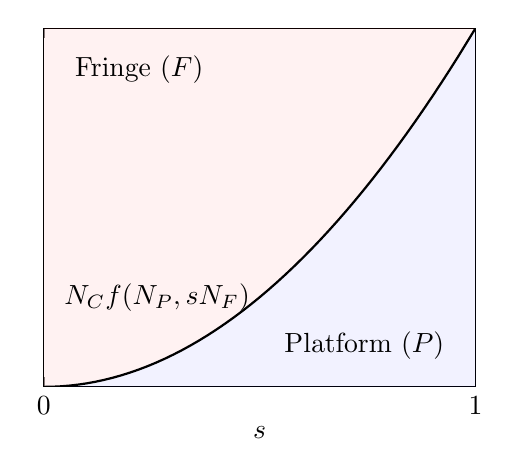
\begin{tikzpicture}[scale=0.8]
            \centering
            \begin{axis}[xmin=0, xmax=1, ymin=0, ymax=1, samples at={0, 0.02, ..., 0.98, 1},
                    xtick={0, 1}, ytick=\empty, xlabel={$s$}]
                \addplot[name path=f, black, thick] {x^2};
                \node[anchor= east] at (axis cs: .5, .5^2) {$N_C f(N_P, sN_F)$};
                \path[name path=bottom] (axis cs:0,0) -- (axis cs:1,0);
                \path[name path=top] (axis cs:0,1) -- (axis cs:1,1);
    
                \addplot [fill=blue, fill opacity=0.05] fill between [of=f and bottom];
                \addplot [fill=red, fill opacity=0.05] fill between [of=f and top];
    
                \node[anchor=north west] at (axis cs: .05, .95) {Fringe ($F$)};
                \node[anchor=south east] at (axis cs: .95, .05) {Platform ($P$)};
            \end{axis}
        \end{tikzpicture}
        \caption{Fringe firms are complements}
    \end{subfigure}
    \begin{subfigure}[b]{0.45\textwidth}
        \centering
        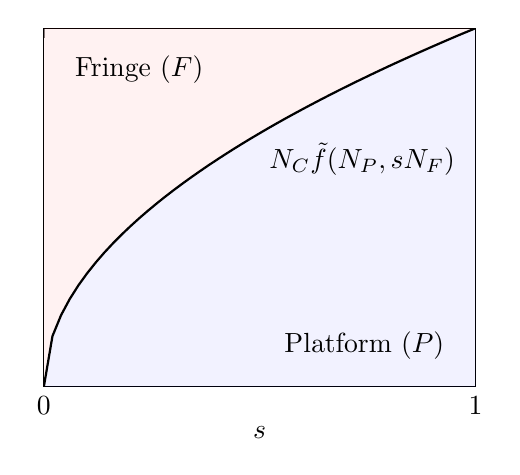
\begin{tikzpicture}[scale=0.8]
            \begin{axis}[xmin=0, xmax=1, ymin=0, ymax=1, samples at={0, 0.02, ..., 0.98, 1},
                xtick={0, 1}, ytick=\empty, xlabel={$s$}]
                \addplot[name path=f, black, thick] {x^0.5};
                \node[anchor=north west] at (axis cs: .5, .5^0.5) {$N_C \tilde{f}(N_P, sN_F)$};
                \path[name path=bottom] (axis cs:0,0) -- (axis cs:1,0);
                \path[name path=top] (axis cs:0,1) -- (axis cs:1,1);
    
                \addplot [fill=blue, fill opacity=0.05] fill between [of=f and bottom];
                \addplot [fill=red, fill opacity=0.05] fill between [of=f and top];
    
                \node[anchor=north west] at (axis cs: .05, .95) {Fringe ($F$)};
                \node[anchor=south east] at (axis cs: .95, .05) {Platform ($P$)};
            \end{axis}
        \end{tikzpicture}
        \caption{Fringe firms are substitutes}
    \end{subfigure}
    \caption{Distribution of value between the platform and the fringe. Profit shares correspond to the shaded areas. The platform's profit share is higher when the fringe firms are more substitutable.}
    \label{fig:outcome_based_bargaining_power}
\end{figure}


\subsection{Entry and equilibrium}

Throughout the paper, I will assume that the number of consumers is fixed and exogenous.
They are thus passive in the sense that they do not make a decision about whether to enter the market or not.
However, when developing microfoundations for $f$ in \cref{sec:example}, consumers will make consumption choices, and their welfare will be of interest.
The product variety of the platform is also exogeneous.

Let us now turn to the determination of the equilibrium number of fringe firms.
Assume that there is an unlimited number of potential fringe entrants, indexed by $i \in \mathbb{R}^+_0$.
In the first stage of the game, each fringe firm must create a viable product at some investment cost.
Let us denote the total investment costs of $N_F$ fringe firms by $I_F(N_F)$.
\begin{assumption}
    Assume that $I_F(N_F)$ is a strictly increasing, convex, twice differentiable function:
    \begin{align*}
        \frac{\partial I_F(N_F)}{\partial N_F} > 0, \quad \frac{\partial^2 I_F(N_F)}{\partial N_F^2} \geq 0.
    \end{align*}
\end{assumption}
This assumption essentially states that the marginal investment cost of the fringe is increasing in the number of fringe firms.
Notice that this only assumes weak convexity, and thus includes the case of constant marginal investment costs.

In the second stage, firms that made this investment plus the platform engage in producing and selling their respective products.
If there are $N_F$ fringe entrants along with $N_P$ platform products and $N_C$ consumers, then, as discussed previously, the total value they create together is given by $\Pi(N_P, N_F, N_C) = N_C f(N_P, N_F)$.
Finally, the platform and the entrants share this profit according to the profit sharing rule from \cref{ass:profit_sharing}, and the fringe gets $\pi_F(N_P, N_F, N_C)$.

The equilibrium number of entrants is determined by a free entry condition: in the end, the fringe firms' total profits should be equal to the aggregated investment cost.
\begin{definition}
    \label{ass:free_entry}
    Let us define a free entry equilibrium by the following conditions:
    \begin{itemize}
        \item Profits are shared according to \cref{ass:profit_sharing}.
        \item Entrants make zero profits after accounting for entry costs: $\pi_F(N_P, N_F) = I_F(N_F)$.
    \end{itemize}
\end{definition}

Finally, in order to guarantee a unique equilibrium, let us make the following, an additional assumption about the profit function.
\begin{assumption}
    \label{ass:single_crossing}
    Let $f$ be such that the following holds for all $N_F, N_P, N_C \geq 0$:
    \begin{align*}
        \frac{\partial \pi_F(N_P, N_F, N_C)}{\partial N_F} < 0 \text{ or } \frac{\partial^2 \pi_F(N_P, N_F, N_C)}{\partial N_F^2} < 0
    \end{align*}
\end{assumption}
This assumption essentially guarantees that the profit of the fringe (as a function of the number of entrants) has at most a single crossing with the --linear -- total entry cost (apart from the obvious $N_F=0$ intersection).
The interpretation of the assumption itself is simple: total fringe profits, as a function of the number of fringe firms, must be either concave or hump-shaped.\footnote{
    As it turns out, even though total industry profits are assumed to be increasing in $n_f$, it is not necessarily true for fringe profits.
    For certain profit functions, it happens that even though the size of the pie increases, the bargaining position of the fringe deteriorates so much that they get a smaller share even in absolute value.
}
What it requires of $f$, however, is not so obvious, and also depends on what one assumes about the innate bargaining weights $w_F$ and $w_P$.
Nevertheless, when microfounding the profit function, one can simply check whether this assumption holds or not.
In particular, it will be satisfied for the logit-type demand in \cref{sec:example}.
% TODO: conjecture: it only has to hold for $f(N_P, N_F)$.


\section{General results}
\label{sec:results}

This section presents some general result that only depend on the abstract model structure described in the previous section, and the assumptions therein.
It turns out that even within such a general setting, one can derive some interesting and non-trivial results.
\Cref{sec:example} then builds on these results to derive stronger ones under a specific demand system.

Let us start with a technical, but very useful result.
\begin{proposition}
    \label{prop:unique_equilibrium}
    Under the conditions in \cref{ass:single_crossing}, the equilibrium is unique if it exists.
\end{proposition}
The intuition behind this result is that \cref{ass:single_crossing} ensures that the total profits achieved by the fringe is either concave or hump-shaped.
Consequently, it has at most one crossing with the -- convex and increasing -- total entry cost function (for $n_F > 0$).
An example for this is shown in \cref{fig:equilibrium}.
This particular shape (concave or hump-shaped) is also the main driver for the later results about the comparative statics of equilibrium profits and entry.

\begin{figure}[ht]
    \centering
    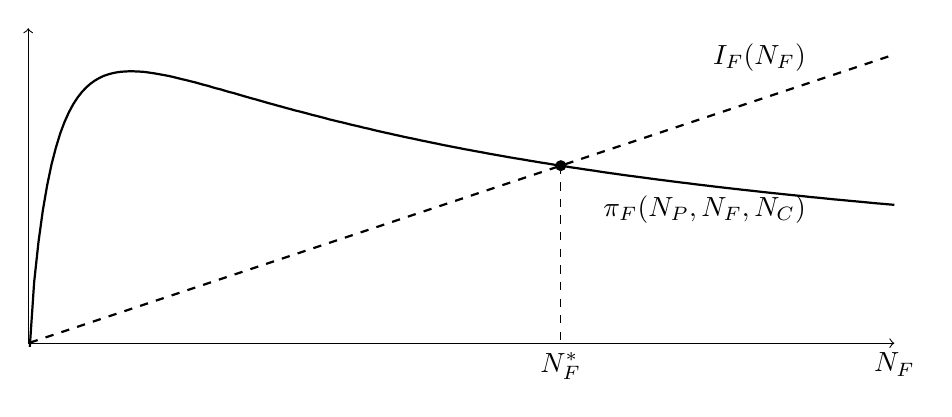
\begin{tikzpicture}[xscale=2,yscale=2,samples=200]
        \draw[->] (0,0) -- (0,2);
        \draw[->] (0,0) -- (5.5,0) node[below] {$N_F$};

        \draw[name path=piF,domain=0.01:5.5,variable=\x,black,thick] plot ({\x},{8*((\x)/(0.3+\x))-8*((\x-0.3*ln(\x+0.3)-0.361)/(\x))});
        \draw[name path=IF,domain=0.01:5.5,variable=\x,black,dashed,thick] plot ({\x},{(\x)/3});
        \node[anchor=north east] at (5,1) {$\pi_F(N_P, N_F, N_C)$};
        \node[anchor=south east] at (5,5/3) {$I_F(N_F)$};

        \fill [name intersections={of=piF and IF, name=i, total=\t}]
            [black] (i-2) circle (1pt);
        \draw[dashed] (i-2) -- (i-2 |- 0,0) node[below] {$N_F^*$};
    \end{tikzpicture}
    \caption{An example free entry equilibrium. \Cref{ass:single_crossing} states that the fringe profit function is concave or hump-shaped in $N_F$, guaranteeing at most one intersection with the linear entry cost function.}
    \label{fig:equilibrium}
\end{figure}

For the following two propositions, let us ignore free entry and equilibrium behavior, and consider the number of fringe entrants $N_F$ as fixed.
The following statement claims that the platform's profits are increasing in its own product variety.
\begin{proposition}
    \label{prop:share_of_platform}
    Assume that $f$ is continuously differentiable with respect to $N_P$ and also twice differentiable.
    Let $N_F \geq 0$.
    Then $\pi_P$ is also differentiable and
    \begin{align*}
        \frac{\partial \pi_P(N_P, N_F)}{\partial N_P} > 0.
    \end{align*}
\end{proposition}
While it might seem obvious, let us still examine what this result does and does not mean.
First, remember that $f$ is increasing in both arguments, and $N_F$ is fixed.
Therefore, an increase in $N_P$ also increases the size of the pie the participants bargain over.
This result states that the slice of the pie that the platform gets increases in this case, too.
It does not mean, however, that the \emph{relative share} of the pie that the platform gets is also bigger -- increase is only guaranteed in absolute terms.
For example, it is possible that for the new, higher value of $N_P$, the complementarities between the fringe firms become stronger, and the platform's bargaining power decreases.\footnote{
    In fact, one can show that this is the case if the cross-derivatives of $f$ are negative.
}
As this result shows, this decrease cannot be large enough to decrease the platform's profits in absolute terms.
\cref{fig:increase_N_P_platform} shows an example of this situation.

\begin{figure}[ht]
    \centering
    \begin{subfigure}[b]{0.45\textwidth}
        \centering
        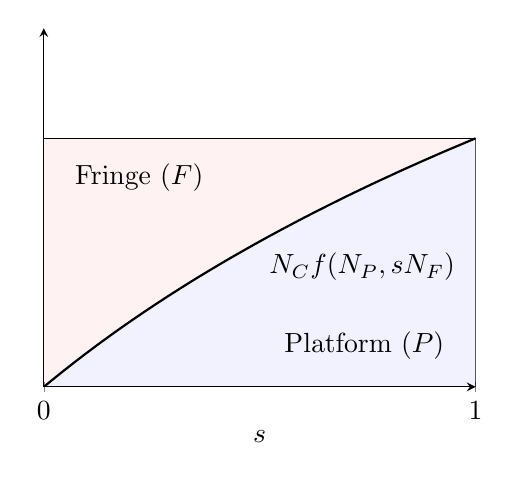
\begin{tikzpicture}[scale=0.8]
            \begin{axis}[xmin=0, xmax=1, ymin=0, ymax=1, samples at={0, 0.02, ..., 0.98, 1},
                xtick={0, 1}, ytick=\empty, axis lines=left, xlabel={$s$}]
                \addplot[name path=f, black, thick] {ln(1+x)};
                % \addplot[name path=tildef, dashed, black] {x};
                \node[anchor=north west] at (axis cs: .5, .4) {$N_C f(N_P, sN_F)$};
                \path[name path=bottom] (axis cs:0,0) -- (axis cs:1,0);
                \draw[name path=top] (axis cs:0,0.693) -- (axis cs:1,0.693);
                \draw[name path=right] (axis cs:1,0) -- (axis cs:1,0.693);
    
                \addplot [fill=blue, fill opacity=0.05] fill between [of=f and bottom];
                \addplot [fill=red, fill opacity=0.05] fill between [of=f and top];
    
                \node[anchor=north west] at (axis cs: .05, .65) {Fringe ($F$)};
                \node[anchor=south east] at (axis cs: .95, .05) {Platform ($P$)};
            \end{axis}
        \end{tikzpicture}
        \caption{Profit shares with $N_P$}
    \end{subfigure}
    \begin{subfigure}[b]{0.45\textwidth}
        \centering
        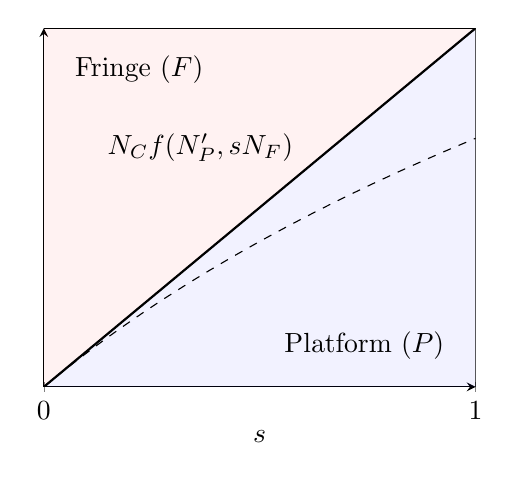
\begin{tikzpicture}[scale=0.8]
            \begin{axis}[xmin=0, xmax=1, ymin=0, ymax=1, samples at={0, 0.02, ..., 0.98, 1},
                xtick={0, 1}, ytick=\empty, axis lines=left, xlabel={$s$}]
                \addplot[name path=f, dashed, black] {ln(1+x)};
                \addplot[name path=tildef, black, thick] {x};
                \node[anchor=south east] at (axis cs: 0.6, 0.6) {$N_C f(N_P', sN_F)$};
                \path[name path=bottom] (axis cs:0,0) -- (axis cs:1,0);
                \draw[name path=top] (axis cs:0,1) -- (axis cs:1,1);
                \draw[name path=right] (axis cs:1,0) -- (axis cs:1,1);
    
                \addplot [fill=blue, fill opacity=0.05] fill between [of=tildef and bottom];
                \addplot [fill=red, fill opacity=0.05] fill between [of=tildef and top];
    
                \node[anchor=north west] at (axis cs: .05, .95) {Fringe ($F$)};
                \node[anchor=south east] at (axis cs: .95, .05) {Platform ($P$)};
            \end{axis}
        \end{tikzpicture}
        \caption{Profit shares with $N_P'$}
    \end{subfigure}
    \caption{Illustration of \cref{prop:share_of_platform} in the one-sided bargaining case. The right hand side figure shows a world with larger platform product variety ($N_P < N_P'$). Even though the platform's share of the total profits is smaller in relative terms in that case, it is still larger in absolute terms.}
    \label{fig:increase_N_P_platform}
\end{figure}

Next, let us look at an analogous result for the fringe firms.
As the next proposition demonstrates, in this case, the direction of the change depends on the complementarities between the fringe firms.
\begin{proposition}
    \label{prop:share_of_fringe}
    Assume that $f, w$ are twice continuously differentiable.
    Let $N_F > 0$.
    Then $\pi_F$ is also differentiable.
    \begin{align*}
        &\text{If } \frac{\partial^2 f(N_P, n_F)}{\partial n_P \partial n_F} < 0 \;\forall n_F \leq N_F, \text{ then } \frac{\partial \pi_F(N_P, N_F)}{\partial N_P} < 0, \\
        &\text{if } \frac{\partial^2 f(N_P, n_F)}{\partial n_P \partial n_F} > 0 \;\forall n_F \leq N_F, \text{ then } \frac{\partial \pi_F(N_P, N_F)}{\partial N_P} > 0
    \end{align*}
    for all $N_P \geq 0$.
\end{proposition}
In summary, when they are mostly substitutes (the cross-derivatives of $f$ are negative), the fringe's profits decrease as a result of an increase in $N_F$.
The intuition is that, even though the total size of the pie increases, the bargaining power of the fringe deteriorates so much that its share decreases not only in relative, but also in absolute terms (as illustrated in \cref{fig:increase_N_P_fringe}).
On the other hand, when the fringe firms are mostly complements the fringe's profits increase.

\begin{figure}[ht]
    \centering
    \begin{subfigure}[b]{0.45\textwidth}
        \centering
        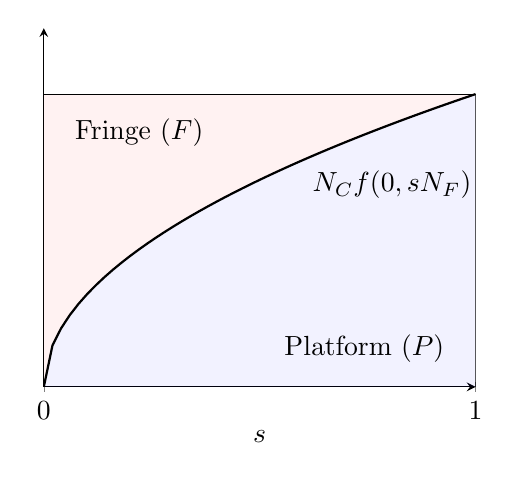
\begin{tikzpicture}[scale=0.8]
            \begin{axis}[xmin=0, xmax=1, ymin=0, ymax=1.225, samples at={0, 0.02, ..., 0.98, 1},
                xtick={0, 1}, ytick=\empty, axis lines=left, xlabel={$s$}]
                \addplot[name path=f, black, thick] {sqrt(x)};
                % \addplot[name path=tildef, dashed, black] {sqrt(0.5+x)};
                \node[anchor=north west] at (axis cs: .6, 0.77) {$N_C f(0, sN_F)$};
                \path[name path=bottom] (axis cs:0,0) -- (axis cs:1,0);
                \draw[name path=top] (axis cs:0,1) -- (axis cs:1,1);
                \draw[name path=right] (axis cs:1,0) -- (axis cs:1,1);
    
                \addplot [fill=blue, fill opacity=0.05] fill between [of=f and bottom];
                \addplot [fill=red, fill opacity=0.05] fill between [of=f and top];
    
                \node[anchor=north west] at (axis cs: .05, .95) {Fringe ($F$)};
                \node[anchor=south east] at (axis cs: .95, .05) {Platform ($P$)};
            \end{axis}
        \end{tikzpicture}
        \caption{Profit shares with $N_P = 0$}
    \end{subfigure}
    \begin{subfigure}[b]{0.45\textwidth}
        \centering
        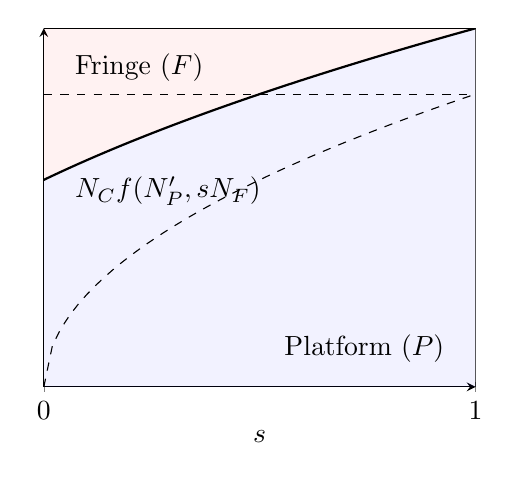
\begin{tikzpicture}[scale=0.8]
            \begin{axis}[xmin=0, xmax=1, ymin=0, ymax=1.225, samples at={0, 0.02, ..., 0.98, 1},
                xtick={0, 1}, ytick=\empty, axis lines=left, xlabel={$s$}]
                \addplot[name path=f, dashed, black] {sqrt(x)};
                \addplot[name path=tildef, black, thick] {sqrt(0.5+x)};
                \node[anchor=north west] at (axis cs: 0.05, 0.75) {$N_C f(N_P', sN_F)$};
                \path[name path=bottom] (axis cs:0,0) -- (axis cs:1,0);
                \draw[name path=top] (axis cs:0,1.225) -- (axis cs:1,1.225);
                \draw[name path=top_old, dashed] (axis cs:0,1) -- (axis cs:1,1);
                \draw[name path=right] (axis cs:1,0) -- (axis cs:1,1.225);
    
                \addplot [fill=blue, fill opacity=0.05] fill between [of=tildef and bottom];
                \addplot [fill=red, fill opacity=0.05] fill between [of=tildef and top];
    
                \node[anchor=north west] at (axis cs: .05, 1.17) {Fringe ($F$)};
                \node[anchor=south east] at (axis cs: .95, .05) {Platform ($P$)};
            \end{axis}
        \end{tikzpicture}
        \caption{Profit shares with $N_P = 0.5$}
    \end{subfigure}
    \caption{Illustration of \cref{prop:share_of_fringe} when fringe and platforrm products are substitutes. An increase in the platform's product variety increases total profits, yet, the fringe's share decreases in absolute terms.}
    \label{fig:increase_N_P_fringe}
\end{figure}

Now let us turn to equilibrium entry as a function of the platform's product variety.
The previous proposition implies an almost immediate corollary regarding the equilibrium number of fringe entrants.
\begin{corollary}
    \label{cor:fringe_entry}
    Assume that $f, w$ are twice continuously differentiable.
    Let $N_F^*$ denote the equilibrium number of fringe firms.
    Let us also assume that $N_F^* > 0$.
    Furthermore, let us assume that
    \begin{align*}
        \frac{\partial^2 f(n_P, n_F)}{\partial n_P \partial n_F} < 0 \quad \forall n_F \leq N_F \\
        \frac{\partial^2 f(n_P, n_F)}{\partial n_F^2} < 0 \quad \forall n_F \leq N_F.
    \end{align*}
    Then the equilibrium number of fringe firms is also differentiable and
    \begin{align*}
        \frac{\partial N_F^*}{\partial N_P} < 0.
    \end{align*}
\end{corollary}
That is, the equilibrium number of entrants increases as a response to an increase in $N_P$ if the fringe firms are mostly complements, and decreases if they are mostly substitutes.
The underlyong reason is again the concave or hump-shaped fringe profit function.
If $N_F^*$ is an equilibrium, then fringe profits minus entry costs are strictly positive for all $N_F \leq N_F^*$ and strictly negative for all $N_F > N_F^*$.
Therefore, if an increase in $N_P$ decreases the fringe's profits for every $N_F \geq 0$, equilibrium can be restored by decreasing the number of fringe entrants, and vice versa for the other case (\cref{fig:comparative_N_F}).

\begin{figure}[ht]
    \centering
    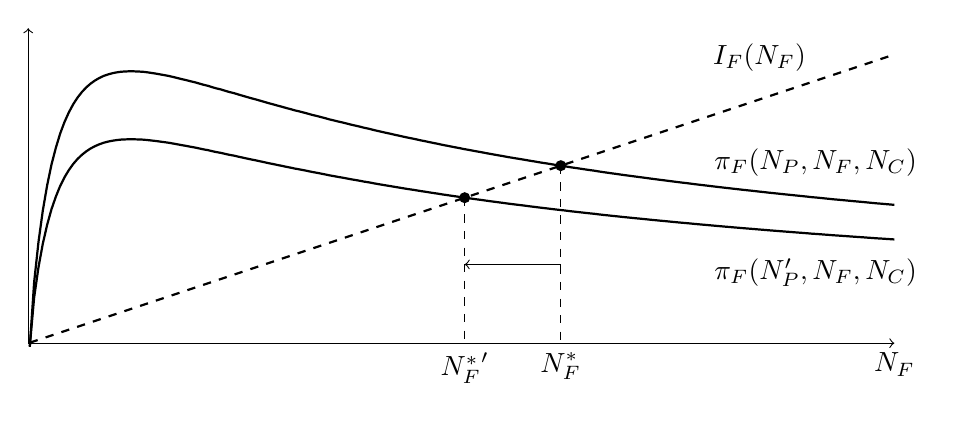
\begin{tikzpicture}[xscale=2,yscale=2,samples=200]
        \draw[->] (0,0) -- (0,2);
        \draw[->] (0,0) -- (5.5,0) node[below] {$N_F$};

        \draw[name path=piF,domain=0.01:5.5,variable=\x,black, thick] plot ({\x},{8*((\x)/(0.3+\x))-8*((\x-0.3*ln(\x+0.3)-0.361)/(\x))});
        \draw[name path=piF2,domain=0.01:5.5,variable=\x,black, thick] plot ({\x},{6*((\x)/(0.3+\x))-6*((\x-0.3*ln(\x+0.3)-0.361)/(\x))});
        \draw[name path=IF,domain=0.01:5.5,variable=\x,black,dashed,thick] plot ({\x},{(\x)/3});

        \node[anchor=south] at (5,1) {$\pi_F(N_P, N_F, N_C)$};
        \node[anchor=north] at (5,0.6) {$\pi_F(N_P', N_F, N_C)$};
        \node[anchor=south east] at (5,5/3) {$I_F(N_F)$};

        \fill [name intersections={of=piF and IF, name=i, total=\t}]
            [black] (i-2) circle (1pt);
        \draw[dashed] (i-2) -- (i-2 |- 0,0) node[below] {$N_F^*$};
        \fill [name intersections={of=piF2 and IF, name=i2, total=\t}]
            [black] (i2-2) circle (1pt);
        \draw[dashed] (i2-2) -- (i2-2 |- 0,0) node[below] {${N_F^*}'$};

        \draw[->] (i-2 |- 0,0.5) -- (i2-2 |- 0,0.5);
    \end{tikzpicture}
    \caption{Illustration of comparative statics for equilibrium entry. If the change in $N_P$ decreases the fringe's profits for every $N_F \geq 0$, equilibrium can be restored by decreasing the number of fringe entrants, and vice versa for the other case.}
    \label{fig:comparative_N_F}
\end{figure}

Finally, let us conclude this section by establishing a stronger result for a more restrictive class of profit functions.
In the following, I assume that the profit function has a specific, additive form.
Intuitively, this means that -- in terms of total profits generated -- the platform's and the fringe firms' products are substitutable to each other according to some constant ratio.
\begin{proposition}
    \label{prop:aggregate_size_additive}
    Let $f$ have the following, additive form:
    \begin{align*}
        f(N_P, N_F) = g(\alpha N_P + \beta N_F)
    \end{align*}
    where $\alpha, \beta > 0$.
    Also assume that $g$ is twice differentiable and that $g'' < 0$.
    Then
    \begin{align*}
        \frac{\partial N_F^*}{\partial N_P} < -\frac{\alpha}{\beta}.
    \end{align*}
    Furthermore,
    \begin{align*}
        \frac{\partial \Pi(N_P, N_F^*(N_P), N_C)}{\partial N_P} < 0.
    \end{align*}
\end{proposition}

The first part of this proposition is a stronger version of \cref{cor:fringe_entry}.
It states that, not only does the equilibrium number of fringe firms decrease as a response to an increase in $N_P$, but it establishes a lower bound for this decrease.
And, as the second part shows, this bound is sufficient to guarantee that the total size of the pie ($\Pi(N_P, N_F, N_C)$) also decreases in equilibrium.

This result has particularly strong implications in models where total profits (or total product variety) has a monotone relationship with consumer welfare, such as those in \textcite{anderson2020aggregative}.
\Cref{sec:example} also presents a demand system which satisfies this property.


\section{Logit demand}
\label{sec:example}

Let us now add more structure to the model, place the function $\Pi$ on more solid microfoundations.
The modeling strategy is heavily inspired by the logit-like demand structure and hybrid platform setting of \textcite{anderson2021hybrid}.
The setting can be thought of as a (possibly hybrid) platform market with monopolistically competing fringe firms.

In the main model, I consider the case when the total profit function only includes the sales of the platform's and fringe firms' products.
That is, the platform does not charge any entry fees to the consumers.
Here, I consider two variants of the model: a benchmark where the platform can unilaterally commit to any entry fee, and a bargaining model where the platform and the fringe firms negotiate over the distribution of profits.
Furthermore, I focus on a particular set of weight functions $w_P$ and $w_F$, which correspont to the Shapley-values of the players in the case of one-sided bargaining.

As an extension, in \cref{sec:lower_bargaining_power} I also examine what happens when the platform and the fringe firms have unequal bargaining weights, while still retaining more structure than the very general bargaining rule from \cref{ass:profit_sharing}.
In particular, I look at the case of bargaining outcomes being described by weighted values, with all fringe players sharing the same weight.
Furthermore, in \cref{sec:two_sided}, I also consider the case of two-sided bargaining, where the consumers also participate in the negotiation over the value produced.
Finally, \cref{sec:total_welfare_one_sided} explores the case of the platform being able to extract all of the consumer surplus through from consumers.

Throughout the analysis, I treat the product variety of the platform and the number of consumers as exogenous, and focus on the equilibrium number of fringe firms.
Nevertheless, the results regarding equilibrium platform profits and consumer surplus are somewhat indicative of the potential general equilibrium behavior of the former two, as well.

\subsection{Setup}

\subsubsection{Demand}

Imagine that there is a unit mass of consumers, looking to buy one product each.
They choose from a continuum of products, indexed by $i$.
Customer $j$ derives the following utility from buying product $i$:
\begin{align*}
    u^F_{ij} = v^F_i - p^F_i + \mu\epsilon^F_{ij},
\end{align*}
where $v^F_i$ is the value of product $i$, $p^F_i$ is its price, and $\epsilon^F_{ij}$ is an idiosyncratic taste shock.
Throughout this section I assume that the value of each product is the same: $v^F_i = v^F$.
This is to simplify the analysis, but is not crucial for the results.

Additionally, customers can also choose from a unit mass of outside options, yielding utility $u^0_ij = \mu\epsilon^0_{ij}$. $\epsilon^F_{ij}$ and $\epsilon^0_{ij}$ are assumed to be independent and identically distributed (i.i.d.) across consumers and products, and follow a standardized Type I Extreme Value distribution. This distributional assumption, along with the fact that each consumer consumes only one product, will lead to a tractable, logit-form demand function.

\subsubsection{Production}

Each (horizontally differentiated) product is produced by a single, monopolistically competitive (fringe) seller.
The production entails a constant marginal cost $c^F_i$.
As with the value, I assume that the marginal cost is the same for all products: $c^F_i = c^F$.
Facing the demand described in the previous paragraphs, the sellers choose their price $p^F_i$ to maximize profits.

Additionally, the platform itself can also offer mass $N_P$ of its own products.
The value and marginal cost of these products are denoted by $v^P$ and $c^P$, respectively.
Furthermore, consumers have the same i.i.d. taste shocks ($\epsilon^P_{ij}$) for platform products as for the products offered by the other sellers.
Finally, I assume that the platform prices its products as if they were produced by separate, monopolistically competitive sellers.
That is, it does not take into account the fact that it can affect a non-zero measure of the prices, and therefore the aggregate demand.
This is to simplify the example, but I expect that it does not affect the main results qualitatively

\subsubsection{Intermediation}

The overall structure of the model comes from \cref{sec:model}: assume that the sellers and the consumers can only interact through an intermediary platform, denoted by $P$.
Without the platform, the fringe firms are not able to sell their products, and thus make no profits.
For this service, the platform can charge a lump-sum entry fee $F_F$ to each fringe firm.\footnote{
    This is a critical difference from \textcite[]{anderson2021hybrid}, where the platform charges a per-unit royalty.
    % TODO: elaborate on this
}
In the baseline model, I assume that entry is free for the consumers, and they are always present on the platform, no matter the other players' entry and pricing decisions.\footnote{
    This essentially means that I assume a one-sided platform, without the usual network effects.
}
Later on, I look at the case of the platform obtaining consumer surplus, and also the case of consumers participating in the bargaining over the total surplus.

As mentioned above, instead of operating as a pure marketplace, the platform may also produce and offer its own products.
Therefore, there are three potential modes of operation.
First, it can offer no product on its own ($N_P = 0$), and operate as a pure marketplace.
Second, it can offer a selection of products alongside with a number of competing fringe firms also being present on the platform ($N_P, N_F > 0$).
In this case, it is a hybrid platform.
Finally, it can operate as a pure retailer, offering its own products, but no products from other sellers ($N_P > 0, N_F = 0$).

\subsubsection{Entry and timing}

There is an infinite measure of fringe firms, who are deciding whether to enter the market.
Entering has two, separate costs: an exogenous investment cost $I_F$, and the platform entry fee $F_F$.
One can conceptualize the first as usual fixed costs, such as the cost of setting up production, or designing a product.
Meanwhile, the second is a payment to the platform for using its services.

In the benchmark model, the game starts by the platform announcing and committing to an entry fee $F_F$.\footnote{
    Without no commitment power, but the ability to set any prices after fringe firms make their investment decisions, the platform would charge an entry fee that would make the fringe profits zero \emph{sans the investment cost}.
    This would lead to a trivial equilibrium, where no firm enters.
}
In the bargaining case, the platform cannot commit to entry fees, so this step is skipped.
Next, each fringe firm decides whether to create a product at cost $I_F$ and enter the market.
% In the bargaining model, the entry fee is decided at this point, as a result of a negotiation between the platform and the firms that have made the investment.
After that, the firms that have made the investment decide if they also want to enter the platform for the announced fee $F_F$.\footnote{
    In the benchmark model, separating these two decisions is redundant, as, in any subgame perfect equilibrium, any firm that makes the investment will also enter the platform.
    However, in the model with bargaining, this distinction is crucial.
}
Finally, the platform and the fringe firms simultaneously choose the prices for their products.
Each consumer then chooses the one maximizing their utility, and profits are realized.

In the baseline model, each player gets their profits from the sales of their products, plus the pre-agreed entry fees from the first period.
In the model with bargaining, the platform and the fringe distribute total profits according to their Shapley values.
One can also think of the latter as agreeing on an entry fee that makes final profits net entry fees equal to the Shapley value of the various players.

The main difference between the benchmark and the bargaining model is in determining the entry fee $F_F$.
In the former, the platform unilaterally sets the fee, and the fringe treats it as a take it or leave it offer.
On the other hand, in the bargaining model, I assume that the entry fee is the result of a negotiation between the parties.


\subsection{Equilibrium}

\subsubsection{Demand and producer profits}

As shown in \textcite[]{anderson2021hybrid}, the utility functions described in \cref{sec:model} give rise to a logit-type demand function.
\begin{proposition}
    \label{prop:demand_function}
    The demand for product $i$ of producer $T \in \{P, F\}$ is given by:
    \begin{align*}
        x_{Ti} = \frac{\exp\left( \frac{v_T - p_{Ti}}{\mu} \right)}{A}
    \end{align*}
    where
    \begin{align}
        A = \int_0^{N_F} \exp\left( \frac{v_F - p_{Fi}}{\mu} \right) \di + \int_0^{N_P} \exp\left( \frac{v_P - p_{Pi}}{\mu} \right) \di + 1.
        \label{eq:aggregate}
    \end{align}
\end{proposition}

Let us call $v_T - p_{Ti}$ the net value of product $i$.
As one would expect, demand is increasing in this net value, and decreasing in the competitors' net values.
Furthermore, demand for each product is increasing in $\mu$, which can be thought of as the degree of product differentiation or the importance of taste shocks.
Finally, notice that, as each producer is infinitesimal, its pricing decision does not affect the aggregate $A$.
This last property makes the optimal prices and profits of the producers very simple, as shown in the next proposition.
\begin{proposition}
    \label{prop:optimal_profit}
    The profit maximizing price for product $Ti$ is
    \begin{align*}
        p^*_{Ti} = c_T + \mu,
    \end{align*}
    and the profit from selling that product is
    \begin{align}
        \pi^{v*}_{Ti} = \mu \frac{\exp \left( \frac{v_T - c_T - \mu}{\mu} \right)}{A}.
        \label{eq:optimal_profit}
    \end{align}
\end{proposition}

For ease of notation, let us define the following:
\begin{align*}
    V_T = \exp \left( \frac{v_T - c_T - \mu}{\mu} \right).
\end{align*}
Then, equilibrium per-product demand and variable profit can be expressed as $V_T/ A$ and $\mu V_T/ A$, respectively, and the total aggregate is simply
\begin{align*}
    A = N_P V_P + N_F V_F + 1.
\end{align*}

Finally, another important feature of this demand system is that, assuming optimal pricing, consumer welfare only depends on the size of the aggregate \parencite{anderson2020aggregative}.
In particular, consumer surplus is proportional to the logarithm of the aggregate: $CS = \mu N_C \log(A)$. This fact makes welfare analysis rather simple in this setting.

\subsubsection{Benchmark: platform sets entry fee unilaterally}

Recall that there is an infinity of potential fringe entrants looking to enter the market.
Therefore, total profits in equilibrium must be zero.
Combined with the  profit function, this gives the following expressions for the equilibrium number of fringe firms and the equilibrium size of the aggregate.
\begin{proposition}
    \label{prop:equilibrium_aggregate}
    If entry costs $I_F$ and $F_F$ are low enough, the equilibrium size of the aggregate is
    \begin{align}
        A = \mu \frac{V_F}{F_F + I_F}.
        \label{eq:aggregate_eq}
    \end{align}
    and the equilibrium number of fringe firms is
    \begin{align*}
        N_F = \frac{\mu}{F_F + I_F} - N_P \frac{V_P}{V_F} - \frac{1}{V_F}.
    \end{align*}
    Otherwise,  $N_F = 0$ and the equilibrium size of the aggregate is
    \begin{align*}
        A = N_P V_P + 1.
    \end{align*}
\end{proposition}
Note that in the first case (\cref{eq:aggregate_eq}), the size of the aggregate does not depend on the platforms' product variety or the platform's product advantage.
The intuition behind this is that per-firm fringe profits only depend on these factors indirectly, through the size of the aggregate.
That is, unless the fringe is not feasible, an increase in $N_P$ will simply replace some fringe entrants, but the free entry condition will pin down the same aggregate, as before.

Now let us turn to the optimal entry fee set by the platform, and its total profits (consisting of revenue from its own sales and the collected entry fees).
The following proposition establishes these both for the hybrid and the pure retail regimes, and \cref{fig:entry_fee,fig:platform_profits} demonstrates them graphically.

\begin{proposition}
    \label{prop:optimal_entry_fee}
    The optimal entry fee is
    \begin{align*}
        F_F^* = \sqrt{\mu I_F V_F} - I_F.
    \end{align*}
    The platform's total profit is
    \begin{align*}
        \pi_P^{t} = \mu - 2\sqrt{\frac{I_F \mu}{V_F}} + \frac{I_F}{V_F} (N_P V_P + 1)
    \end{align*}
    in the hybrid regime, and
    \begin{align*}
        \pi_P^{t} = \pi_P^{v} = \mu \frac{ N_P V_P}{N_P V_P + 1}
    \end{align*}
    in the retail regime.
\end{proposition}
Note, that even though the platform's profit is increasing in the number of its products, the optimal entry fee does not depend on it (\cref{fig:platform_profits,fig:entry_fee}).
This is only due to the fact that the platform's product does not require any investment cost.
If the platform is operating in the hybrid regime, less fringe firms are needed to achieve the (fixed) equilibrium aggregate, therefore there is less expenditure on investment costs, which is essentially wasted.
Consequently, in the hybrid regime, the marginal derivative of optimal profits with respect to the platform's product variety is simply the fringe's investment cost, adjusted for the possible difference in product advantage:
\begin{align*}
    N_F > 0 \implies \frac{\partial \pi_P^t}{\partial N_P} = \frac{V_P}{V_F} I_F.
\end{align*}
Furthermore, if the platform does have to pay an investment cost $I_P$, then it will only have its own products if $\frac{I_P}{V_P} \leq \frac{I_F}{V_F}$, which is efficient from a welfare perspective.

As a consequence, as long as the fringe is feasible at the optimal entry fee, the size of the aggregate, and hence consumer welfare is also unaffected by the platform operating in hybrid mode.
In contrast, when the fringe is not present in the market, total aggregate, and hence consumer welfare are increasing in the number of the platform's products.
This effect is purely mechanical: more variety leads to higher welfare.
\Cref{fig:fringe_entry_eq} illustrates this effect.

Finally, note that the profit of the platform under the hybrid regime is higher than under the retail regime, whenever the former is feasible.
Therefore, for a given $N_P$, the platform prefers to operate in hybrid mode, and does not want to exclude fringe firms from the market.
As a corollary, in the benchmark model, a platform becoming a hybrid platform, or increasing the number of its own products, always has a weakly positive effect on the aggregate, and thus consumer welfare.\footnote{
    This is in contrast to \textcite{anderson2021hybrid}, where a platform operating in hybrid mode sets higher royalties to create a price advantage for its own products.
    The reason for this difference lies in the type of entry fee: they assume a revenue-based, proportional fee, which distorts prices.
    In contrast, in this paper, I assume a non-distortive lump sum fee.
}
\subsubsection{Main model: bargaining between platform and fringe}

Now consider the case where, instead of the platform setting take it or leave it entry fees, it must negotiate with the fringe about the division of profits.
As the platform cannot choose and commit to an entry fee, the first period from the benchmark model is skipped.
Instead, the game starts by fringe firms' investment decisions.
After that, in the second period, bargaining takes place between the platform and the fringe firms that have entered the market.

The participants negotiate over the aggregate profits that they expect to obtain in the subsequent period (assuming the same non-collusive, monopolistic pricing, as before).
I assume that bargaining outcomes are determined according to \cref{ass:profit_sharing}, where $\Pi(N_P, N_F, N_C)$ is defined as the sum of profits that the platform and the entrants acquire by selling their products.
From \cref{eq:optimal_profit}, the total profit achieved by the platform and $N_F$ fringe firms is given by
\begin{align*}
    \Pi(N_P, N_F, N_C) = N_C \underbracket{\mu \frac{n V_F + N_P V_P}{n V_F + N_P V_P + 1}}_{\coloneqq f(N_P, N_F)}.
\end{align*}

Let us assume that the bargaining results in profits being shared according to players' Shapley values.
These Shapley values satisfy \cref{ass:profit_sharing}, with $w_P(s) \equiv 1$ and $w_F(s) = s$.\footnote{
    For a discussion and proof of this claim, see \cref{sec:cooperative_game}.
}
Based on these, one can even obtain closed-form expressions for platform and fringe profit shares for this class of demand systems.
\begin{proposition}
    \label{prop:platform_profits_bargaining}
    The platform's total profits are
    \begin{align*}
        \pi^t_P &= N_C \int_0^1 f(N_P, sN_F) \ds \\
                &= \mu N_C \left[ 1 - \frac{\log \left(1 + \frac{N_F V_F}{N_P V_P + 1} \right)}{N_F V_F} \right].
    \end{align*}
    The total profits of the whole fringe (including investment costs) are given by
    \begin{align*}
        \pi^t_F = \mu N_C \left[ \frac{\log \left( 1 + \frac{N_F V_F}{N_P V_P + 1} \right)}{N_F V_F} - \frac{1}{N_P V_P + N_F V_F + 1} \right] - I_F N_F .
    \end{align*}
\end{proposition}

Now let us turn to how the platform's dual mode operation affects product variety and consumer welfare.
I will rely on results from \cref{sec:results} to establish comparative statics for the equilibrium aggregate.
Let us start by showing that $f(n_P, n_F)$ satisfies the assumptions those results rely on.
\begin{lemma}
    \label{lem:profit_assumptions}
    $f(n_P, n_F)$ satisfies \cref{ass:single_crossing}.
    Furthermore,
    \begin{align*}
        \frac{\partial^2 f(n_P, n_F)}{\partial n_P \partial n_F} < 0.
    \end{align*}
\end{lemma}
Using this, \cref{prop:unique_equilibrium} gives that the equilibrium is unique.
Furthermore, \cref{cor:fringe_entry} implies that an increase in the number of the platform's products leads to a reduction in the number of fringe firms that enter the market.

Owing to the additive nature of the total profit function, an even stronger result can be obtained.
Notice that $f$ has the functional form required for proposition \ref{prop:aggregate_size_additive} with $g(x) = \frac{x}{1+x}, \alpha = V_P, \beta = V_F$.
Therefore, the same proposition implies that
\begin{align*}
    \frac{\partial N_F^*}{\partial N_P} < -\frac{V_P}{V_F},
\end{align*}
that is, an increase in the platform's products leads to a more than proportional reduction in the number of fringe products (\cref{fig:fringe_entry_eq}).

As a consequence of this, equilibrium total aggregate is also decreasing in $N_P$.\footnote{
    The same result also holds true for an increase in the paltform's product advantage $V_P$.
}
As, in this model, consumer welfare is monotone in the total aggregate, this implies that consumer welfare is decreasing in the number of the platform's products (\cref{fig:welfare}).
Therefore, as opposed to the benchmark model, the platform becoming more hybrid leads to a reduction in consumer welfare.\footnote{
    Unless $V_P N_P$ is high enough that the platform would operate in pure retail mode in the benchmark model, too.
}

The intuition behind this is demonstrated in can be captured by looking at entry fees.
First, define the implied entry fee in the bargaining case as the difference between the variable profit and the final, total profit of the fringe firms, less the investment cost:
\begin{align*}
    F_F^{\text{impl}} = \pi_F^v - \pi_F^t + I_F.
\end{align*}
As shown before, the platform's product variety grows, its bargaining power also increases.
This can be thought of as an increase in (implied) entry fees $F_F^{\text{impl}}$, which in turn discourages fringe entry \cref{fig:entry_fee}.

In this specific demand system and parametrization, the implied entry fee is higher than what the platform would prefer to set for any $N_P \geq 0$.
If it could, it would commit to a lower entry fee to incentivize more fringe entry, and thus increase total profits.
This is an example that bargaining instead of unilateral pricing does not necessarily lead to lower platform shares, or better welfare outcomes: it can be a lose-lose situation for both the platform and the consumers.
\Cref{sec:lower_bargaining_power} explores an alternative model where the platform has less bargaining power, and thus -- for sufficiently low values of $N_P$ -- the implied entry fee it achieves in the bargaining model is lower than what it would set unilaterally.

Finally, let us look at the platform's profits in equilibrium.
As in the benchmark model, they are increasing in the number platform's product variety $N_P$ (\cref{fig:platform_profits}). % TODO: can I make it a proper proposition?
However, in contrast to that case, there is an important difference in the hybrid regime.
In the benchmark model, the entry fee was independent of the platform's product variety.
On the other hand, with bargaining, it is increasing in $N_P$ (\cref{fig:entry_fee}).
Therefore, if the entry fee is already higher than optimal for a given $N_P$, an additional increase will lead to an even more suboptimal (implied) entry fee, and thus a lower increase in platform profits than it would otherwise.
This is the case in the example parametrization displayed on the figures for every $N_P \geq 0$.

This means that, if the platform had to create its product variety at a per-unit investment cost of $I_P$, it would make different (inefficient) choices compared to the benchmark model.
In particular, it might invest in some products even if it has a product disadvantage, and it might not invest in some products even if it has a product disadvantage.
This phenomenon is more pronounced when the implied entry fee for $N_P = 0$ is lower than optimal, and is explored in more detail in \cref{sec:lower_bargaining_power}.

\begin{figure}
    \centering
    \begin{subfigure}[b]{0.45\textwidth}
        \centering
        \begin{tikzpicture}
            \begin{axis}[
                    xlabel={$N_P$},
                    xmin=0, xmax=1.5, % adjust these values as needed
                    ymin=0, ymax=1.4, % adjust these values as needed
                    width=\linewidth, % adjust the width of the plot
                    axis lines=left,
                    xtick={0, 1.5},
                ]
                \addplot[color=myblue,mark=none,thick] table[x=N_P,y=N_F_bench]{\equilibrium};
                \addplot[color=myred,mark=none,thick] table[x=N_P,y=N_F]{\equilibrium};
                \legend{Benchmark, Bargaining}

                \addplot[draw=none,name path=hybrid] table[x=N_P,y=hybrid]{\equilibrium};
                \addplot[draw=none,name path=hybrid_bench] table[x=N_P,y=hybrid_bench]{\equilibrium};
                \addplot[draw=none,name path=bottom] {0};
                \addplot [fill=black, fill opacity=0.05] fill between [of=hybrid and bottom];
                \addplot [fill=black, fill opacity=0.05] fill between [of=hybrid_bench and bottom];
            \end{axis}
        \end{tikzpicture}
        \caption{Equilibrium number of fringe firms ($N_F$)}
        \label{fig:fringe_entry_eq}
    \end{subfigure}
    \hfill
    \begin{subfigure}[b]{0.45\textwidth}
        \centering
        \begin{tikzpicture}
            \begin{axis}[
                    xlabel={$N_P$},
                    ylabel={$F_F$},
                    xmin=0, xmax=1.5, % adjust these values as needed
                    ymin=0, ymax=0.65, % adjust these values as needed
                    width=\linewidth, % adjust the width of the plot
                    axis lines=left,
                    xtick={0, 1.5},
                    legend pos=north east
                ]
                \addplot[color=myblue,mark=none,thick] table[x=N_P,y=F_F_opt]{\equilibrium};
                \addplot[color=myred,mark=none,thick] table[x=N_P,y=F_F_implied]{\equilibrium};
                \legend{Benchmark, Bargaining (implied)}

                \addplot[draw=none,name path=hybrid] table[x=N_P,y=hybrid]{\equilibrium};
                \addplot[draw=none,name path=hybrid_bench] table[x=N_P,y=hybrid_bench]{\equilibrium};
                \addplot[draw=none,name path=bottom] {0};
                \addplot [fill=black, fill opacity=0.05] fill between [of=hybrid and bottom];
                \addplot [fill=black, fill opacity=0.05] fill between [of=hybrid_bench and bottom];
            \end{axis}
        \end{tikzpicture}
        \caption{Optimal/implied entry fee ($F_F$)}
        \label{fig:entry_fee}
    \end{subfigure}
    \caption{Equilibrium number of fringe entrants and (implied) entry fees ($\mu = 1, N_C = 1, V_P = 1, V_F = 1, I_F = 0.2$). In the benchmark model, the entry fee does not depend on the platform's product variety, and an increase in $N_P$ leads to a proportional reduction in $N_F$. In contrast, in the bargaining case, the entry fee is increasing in $N_P$, and the reduction in $N_F$ is more than proportional. Dark shaded area represents hybrid mode under the bargaining assumption, while light shaded area represents additional hybrid mode under the benchmark assumption.}
    \label{fig:entry_and_fees}
\end{figure}


\begin{figure}
    \centering
    \begin{tikzpicture}
        \begin{axis}[
                xlabel={$N_P$},
                    xmin=0, xmax=1.5, % adjust these values as needed
                    ymin=0, ymax=0.65, % adjust these values as needed
                    width=0.5\linewidth, % adjust the width of the plot
                    axis lines=left,
                    xtick={0, 1.5},
                    legend pos=south east
                ]
            \addplot[color=myblue,mark=none,thick] table[x=N_P,y=pi_P_bench]{\equilibrium};
            \addplot[color=myred,mark=none,thick] table[x=N_P,y=pi_P]{\equilibrium};
            \addplot[color=black,mark=none,thick,dashed] table[x=N_P,y=pi_P_noF]{\equilibrium};
            \legend{Benchmark, Bargaining, Pure retail}

            \addplot[draw=none,name path=hybrid] table[x=N_P,y=hybrid]{\equilibrium};
            \addplot[draw=none,name path=hybrid_bench] table[x=N_P,y=hybrid_bench]{\equilibrium};
            \addplot[draw=none,name path=bottom] {0};
            \addplot [fill=black, fill opacity=0.05] fill between [of=hybrid and bottom];
            \addplot [fill=black, fill opacity=0.05] fill between [of=hybrid_bench and bottom];
        \end{axis}
    \end{tikzpicture}
    \caption{Platform profits in equilibrium ($\mu = 1, N_C = 1, V_P = 1, V_F = 1, I_F = 0.2$). In both cases, platform profits are increasing in $N_P$. However, in the case of the hybrid regime under bargaining, this increase is lower, due to the fact that prices deviate further from optimal. Dark shaded area represents hybrid mode under the bargaining assumption, while light shaded area represents additional hybrid mode under the benchmark assumption.}
    \label{fig:platform_profits}
\end{figure}

\begin{figure}
    \centering
    \begin{subfigure}[b]{0.45\textwidth}
        \centering
        \begin{tikzpicture}
            \begin{axis}[
                    xlabel={$N_P$},
                    xmin=0, xmax=1.5, % adjust these values as needed
                    ymin=0, ymax=3, % adjust these values as needed
                    width=\linewidth, % adjust the width of the plot
                    axis lines=left,
                    xtick={0, 1.5},
                    legend pos=south east
                ]
                \addplot[color=myblue,mark=none,thick] table[x=N_P,y=A_bench]{\equilibrium};
                \addplot[color=myred,mark=none,thick] table[x=N_P,y=A]{\equilibrium};
                \addplot[color=black,mark=none,thick,dashed] table[x=N_P,y=A_noF]{\equilibrium};
                \legend{Benchmark, Bargaining, Pure retail}

                \addplot[draw=none,name path=hybrid] table[x=N_P,y=hybrid]{\equilibrium};
                \addplot[draw=none,name path=hybrid_bench] table[x=N_P,y=hybrid_bench]{\equilibrium};
                \addplot[draw=none,name path=bottom] {0};
                \addplot [fill=black, fill opacity=0.05] fill between [of=hybrid and bottom];
                \addplot [fill=black, fill opacity=0.05] fill between [of=hybrid_bench and bottom];
            \end{axis}
        \end{tikzpicture}
        \caption{Aggregate ($A$)}
    \end{subfigure}
    \hfill
    \begin{subfigure}[b]{0.45\textwidth}
        \centering
        \begin{tikzpicture}
            \begin{axis}[
                    xlabel={$N_P$},
                    xmin=0, xmax=1.5, % adjust these values as needed
                    ymin=0, ymax=1.5, % adjust these values as needed
                    width=\linewidth, % adjust the width of the plot
                    axis lines=left,
                    xtick={0, 1.5},
                    legend pos=south east
                ]
                \addplot[color=myblue,mark=none,thick] table[x=N_P,y=CS_bench]{\equilibrium};
                \addplot[color=myred,mark=none,thick] table[x=N_P,y=CS]{\equilibrium};
                \addplot[color=black,mark=none,thick,dashed] table[x=N_P,y=CS_noF]{\equilibrium};
                \legend{Benchmark, Bargaining, Pure retail}

                \addplot[draw=none,name path=hybrid] table[x=N_P,y=hybrid]{\equilibrium};
                \addplot[draw=none,name path=hybrid_bench] table[x=N_P,y=hybrid_bench]{\equilibrium};
                \addplot[draw=none,name path=bottom] {0};
                \addplot [fill=black, fill opacity=0.05] fill between [of=hybrid and bottom];
                \addplot [fill=black, fill opacity=0.05] fill between [of=hybrid_bench and bottom];
            \end{axis}
        \end{tikzpicture}
        \caption{Consumer surplus ($CS$)}
    \end{subfigure}
    \caption{Size of the aggregate and consumer surplus in equilibrium ($\mu = 1, N_C = 1, V_P = 1, V_F = 1, I_F = 0.2$). In the benchmark model, an increase in platform product variety has no effect in the hybrid regime. Under bargaining, it does have a negative effect on total product variety, and, in turn, consumer surplus. The increase has a (mechanical) positive effect in the pure retail regime under both assumptions. Dark shaded area represents hybrid mode under the bargaining assumption, while light shaded area represents additional hybrid mode under the benchmark assumption.}
    \label{fig:welfare}
\end{figure}


\section{Extensions}

\subsection{Platform has lower innate bargaining power}
\label{sec:lower_bargaining_power}

In the previous sections, I assumed that the platform and the fringe firms split total profits according to their Shapley values.
Because of the symmetry property of the Shapley value, this excludes the possibility of players having some kind of innate bargaining power, which is not related to the profit functions.
In this extension, I will relax this assumption, and assume instead that profits are shared according to \emph{weighed} Shapley values.
These are a generalization of the Shapley value, where each player has a weight $w_i$ that can, in certain settings, be thought of as a parameter describing bargaining power.\footnote{
    \textcite{hart1996bargaining} and \textcite{stole1996intra} provide foundations for this interpretation.
}
Similarly to the standard Shapley value, one can show that outcomes based on weighted values also satisfy \cref{ass:profit_sharing}.
Specifically, when the weight of the platform is $\lambda_P$, the functions $w_P$ and $w_F$ are given by
\begin{align*}
    w_P(s) &= \lambda_P s ^ {\lambda_P - 1} \\
    w_F(s) &= s ^ {\lambda_P}.
\end{align*}

\textcolor{red}{TODO: can I show that \cref{ass:single_crossing} still holds for any $\lambda_P$? If not, focus on a specific case, such as the one on the graphs.}

The example parametrizatrion is the same as in the main model, with the only difference that the platform has a lower innate bargaining power ($\lambda_P = 0.5$).
As the conditions in \cref{ass:single_crossing} are also satisfied in this case, the main observations from \cref{sec:results} also apply.
That is, as shown on \cref{fig:fringe_entry_eq_low_lambda}, total aggregate is decreasing in $N_P$ throughout the hybrid regime, due to the platform's products displacing more fringe products than their total number.

The main difference is that, due to the lower bargaining power of the platform, the implied entry fee (\cref{fig:platform_profits_low_lambda}) is lower than the benchmark, unilaterally set one for low enough $N_P$.
As a consequence, total aggregate, and thus consumer surplus, is also above the benchmark outcome in that case.
Furthermore, there exists some $\bar{N}_P$ for which the unilateral price setting and bargaining outcomes coincide in terms of all variables, due to the implied entry fee being the same.

Another major difference pertains to the total profits of the platform as a function of $N_P$.
It is still true that they are increasing in the number of the platform's products, but now this increase is even more pronounced for low values of $N_P$.
The reason is that for low $N_P$, the implied entry fee is lower than the optimal one.
Furthermore, it increases in $N_P$ as a result of the platform's increased bargaining power.
Therefore, the platform's profits are increasing in $N_P$ even more than in the benchmark case or the main model, up to the point where the implied entry fee is equal to the optimal one.
After that, the same effect as in the main model kicks in, and the increase in profits is lower than in the benchmark case.

\Cref{fig:equilibrium_low_lambda_entry_fees} demonstrates an important consequence of this phenomenon.
Imagine that the platform can decide on the number of its products at time 0, at an investment cost of $I_P$ per product.
In the main model, due to the implied entry fee being higher than optimal even for $N_P = 0$, hybrid operation is never optimal.
The platform would always prefer either pure retail or pure marketplace operation.
In contrast, when the platform has lower bargaining power, there exists a range of $I_P$ values (e.g. $I_P = 0.2$) for which the platform would prefer to operate in hybrid mode.
Furthermore, if hybrid operation is not allowed, the platform might switch to become a pure marketplace, thereby increasing consumer surplus.


\begin{figure}
    \centering
    \begin{subfigure}[b]{0.45\textwidth}
        \centering
        \begin{tikzpicture}
            \begin{axis}[
                    xlabel={$N_P$},
                    xmin=0, xmax=1.5, % adjust these values as needed
                    ymin=0, ymax=1.8, % adjust these values as needed
                    width=\linewidth, % adjust the width of the plot
                    axis lines=left,
                    xtick={0, 1.5},
                ]
                \addplot[color=myblue,mark=none,thick] table[x=N_P,y=N_F_bench]{\equilibrium};
                \addplot[color=myred,mark=none,thick] table[x=N_P,y=N_F]{\equilibrium};
                \addplot[color=mygreen,mark=none,thick] table[x=N_P,y=N_F]{\equilibriumProfitOneSidedLowLambda};
                \legend{Benchmark, Bargaining ($\lambda = 1$), Bargaining ($\lambda = 0.5$)}

                \addplot[draw=none,name path=hybrid] table[x=N_P,y=hybrid]{\equilibrium};
                \addplot[draw=none,name path=hybrid_alt] table[x=N_P,y=hybrid]{\equilibriumProfitOneSidedLowLambda};
                \addplot[draw=none,name path=bottom] {0};
                \addplot [fill=black, fill opacity=0.05] fill between [of=hybrid and bottom];
                \addplot [fill=black, fill opacity=0.05] fill between [of=hybrid_alt and bottom];
            \end{axis}
        \end{tikzpicture}
        \caption{Equilibrium number of fringe firms ($N_F$)}
        \label{fig:fringe_entry_eq_low_lambda}
    \end{subfigure}
    \hfill
    \begin{subfigure}[b]{0.45\textwidth}
        \centering
        \begin{tikzpicture}
            \begin{axis}[
                    xlabel={$N_P$},
                    xmin=0, xmax=1.5, % adjust these values as needed
                    ymin=0, ymax=3, % adjust these values as needed
                    width=\linewidth, % adjust the width of the plot
                    axis lines=left,
                    xtick={0, 1.5},
                    legend pos=south east,
                ]
                \addplot[color=myblue,mark=none,thick] table[x=N_P,y=A_bench]{\equilibrium};
                \addplot[color=myred,mark=none,thick] table[x=N_P,y=A]{\equilibrium};
                \addplot[color=mygreen,mark=none,thick] table[x=N_P,y=A]{\equilibriumProfitOneSidedLowLambda};
                \legend{Benchmark, Bargaining ($\lambda = 1$), Bargaining ($\lambda = 0.5$)}

                \addplot[draw=none,name path=hybrid] table[x=N_P,y=hybrid]{\equilibrium};
                \addplot[draw=none,name path=hybrid_alt] table[x=N_P,y=hybrid]{\equilibriumProfitOneSidedLowLambda};
                \addplot[draw=none,name path=bottom] {0};
                \addplot [fill=black, fill opacity=0.05] fill between [of=hybrid and bottom];
                \addplot [fill=black, fill opacity=0.05] fill between [of=hybrid_alt and bottom];
            \end{axis}
        \end{tikzpicture}
        \caption{Equilibrium number of fringe firms ($N_F$)}
    \end{subfigure}
    \caption{Equilibrium outcomes in the case when the platform has lower innate bargaining power ($N_C = 1, V_P = 1, V_F = 1, I_F = 0.2$). As in every other case, the platform's profits are increasing in $N_P$, while the fringe's profits are decreasing. Furthermore, consumer surplus is also decreasing as a result in a decrease in total product variety. The shaded region represents hybrid operation, while in the unshaded region, the platform operates in pure retail mode.}
    \label{fig:equilibrium_low_lambda}
\end{figure}


\begin{figure}
    \centering
    \begin{subfigure}[b]{0.45\textwidth}
        \centering
        \begin{tikzpicture}
            \begin{axis}[
                    xlabel={$N_P$},
                    ylabel={},
                    xmin=0, xmax=1.5, % adjust these values as needed
                    ymin=0, ymax=0.65, % adjust these values as needed
                    axis lines=left,
                    xtick={0, 1.5},
                    legend pos=south east,
                    width=\linewidth,
                ]
                \addplot[color=myblue,mark=none,thick] table[x=N_P,y=pi_P_bench]{\equilibrium};
                \addplot[color=myred,mark=none,thick] table[x=N_P,y=pi_P]{\equilibrium};
                \addplot[color=mygreen,mark=none,thick] table[x=N_P,y=pi_P]{\equilibriumProfitOneSidedLowLambda};
                \addplot[color=black,mark=none,thick,dashed] table[x=N_P,y=pi_P_noF]{\equilibrium};

                \legend{Benchmark, Bargaining ($\lambda = 1$), Bargaining ($\lambda = 0.5$)}
                
                \addplot[draw=none,name path=hybrid] table[x=N_P,y=hybrid]{\equilibriumProfitOneSidedLowLambda};
                \addplot[draw=none,name path=hybrid_orig] table[x=N_P,y=hybrid]{\equilibrium};
                \addplot[draw=none,name path=bottom] {0};
                \addplot [fill=black, fill opacity=0.05] fill between [of=hybrid and bottom];
                \addplot [fill=black, fill opacity=0.05] fill between [of=hybrid_orig and bottom];
            \end{axis}
        \end{tikzpicture}
        \caption{Platform profits}
        \label{fig:platform_profits_low_lambda}
    \end{subfigure}
    \hfill
    \begin{subfigure}[b]{0.45\textwidth}
        \centering
        \begin{tikzpicture}
            \begin{axis}[
                    xlabel={$N_P$},
                    ylabel={},
                    xmin=0, xmax=1.5, % adjust these values as needed
                    ymin=0, ymax=0.5, % adjust these values as needed
                    axis lines=left,
                    xtick={0, 1.5},
                    legend pos=south east,
                    width=\linewidth,
                ]
                \addplot[color=myblue,mark=none,thick] table[x=N_P,y=F_F_opt]{\equilibrium};
                \addplot[color=myred,mark=none,thick] table[x=N_P,y=F_F_implied]{\equilibrium};
                \addplot[color=mygreen,mark=none,thick] table[x=N_P,y=F_F_implied]{\equilibriumProfitOneSidedLowLambda};

                \legend{Benchmark, Bargaining ($\lambda = 1$), Bargaining ($\lambda = 0.5$)}
                
                \addplot[draw=none,name path=hybrid] table[x=N_P,y=hybrid]{\equilibriumProfitOneSidedLowLambda};
                \addplot[draw=none,name path=hybrid_orig] table[x=N_P,y=hybrid]{\equilibrium};
                \addplot[draw=none,name path=bottom] {0};
                \addplot [fill=black, fill opacity=0.05] fill between [of=hybrid and bottom];
                \addplot [fill=black, fill opacity=0.05] fill between [of=hybrid_orig and bottom];
            \end{axis}
        \end{tikzpicture}
        \caption{Optimal/implied entry fee}
        \label{fig:entry_fee_low_lambda}
    \end{subfigure}
    \caption{Platform profits and (implied) entry fees ($\mu = 0.2, N_C = 1, V_P = 1, V_F = 1, I_F = 0.2$). Regardless of lambda, platform profits and entry fees are increasing in $N_P$. However, when the platform's innate bargaining power is higher, entry fees are above optimal levels already for $N_P = 0$, and the additional increase somewhat mitigates the benefits of the platform's increased product variety. When $\lambda$ is lower, the entry fees are below optimal for low $N_P$, therefore increasing $N_P$ has a larger positive effect on profits. Dark shaded area represents hybrid mode under $\lambda=1$, while light shaded area represents additional hybrid mode under $\lambda=0.5$.}
    \label{fig:profits_and_entry_fees_low_lambda}
\end{figure}


\begin{figure}
    \centering
    \begin{subfigure}[b]{0.45\textwidth}
        \centering
        \begin{tikzpicture}
            \begin{axis}[
                    xlabel={$N_P$},
                    ylabel={},
                    xmin=0, xmax=1.5, % adjust these values as needed
                    ymin=0.2, ymax=0.35, % adjust these values as needed
                    axis lines=left,
                    xtick={0, 1.5},
                    legend pos=north west,
                    width=\linewidth,
                ]
                \addplot[color=myblue,mark=none,thick] table[x=N_P,y expr=\thisrow{pi_P} - \thisrow{N_P} * 0.18]{\equilibrium};
                \addplot[color=myred,mark=none,thick] table[x=N_P,y expr=\thisrow{pi_P} - \thisrow{N_P} * 0.2]{\equilibrium};
                \addplot[color=mygreen,mark=none,thick] table[x=N_P,y expr=\thisrow{pi_P} - \thisrow{N_P} * 0.22]{\equilibrium};

                \addplot[draw=none,name path=hybrid] table[x=N_P,y=hybrid]{\equilibrium};
                \addplot[draw=none,name path=bottom] {0};
                \addplot [fill=black, fill opacity=0.05] fill between [of=hybrid and bottom];

                \legend{$I_P = 0.18$, $I_P = 0.2$, $I_P = 0.22$}
            \end{axis}
        \end{tikzpicture}
        \caption{$\lambda = 1$}
    \end{subfigure}
    \hfill
    \begin{subfigure}[b]{0.45\textwidth}
        \centering
        \begin{tikzpicture}
            \begin{axis}[
                    xlabel={$N_P$},
                    ylabel={},
                    xmin=0, xmax=1.5, % adjust these values as needed
                    ymin=0.2, ymax=0.35, % adjust these values as needed
                    axis lines=left,
                    xtick={0, 1.5},
                    legend pos=south west,
                    width=\linewidth,
                ]
                \addplot[color=myblue,mark=none,thick] table[x=N_P,y expr=\thisrow{pi_P} - \thisrow{N_P} * 0.18]{\equilibriumProfitOneSidedLowLambda};
                \addplot[color=myred,mark=none,thick] table[x=N_P,y expr=\thisrow{pi_P} - \thisrow{N_P} * 0.2]{\equilibriumProfitOneSidedLowLambda};
                \addplot[color=mygreen,mark=none,thick] table[x=N_P,y expr=\thisrow{pi_P} - \thisrow{N_P} * 0.22]{\equilibriumProfitOneSidedLowLambda};

                \addplot[draw=none,name path=hybrid] table[x=N_P,y=hybrid]{\equilibriumProfitOneSidedLowLambda};
                \addplot[draw=none,name path=bottom] {0};
                \addplot [fill=black, fill opacity=0.05] fill between [of=hybrid and bottom];

                \legend{$I_P = 0.18$, $I_P = 0.2$, $I_P = 0.22$}
            \end{axis}
        \end{tikzpicture}
        \caption{$\lambda = 0.5$}
    \end{subfigure}
    \caption{Total platform profits if the platform incurs an investment cost for creating its own products ($\pi_P(N_P) - I_P N_P$). In the high bargaining power case (left), the platform never chooses to operate in hybrid mode. It either becomes a pure marketplace or a pure retailer. In the case of lower $\lambda_P$ (right), choosing the hybrid mode can be optimal depending on $I_P$. The shaded region represents hybrid operation, while in the unshaded region, the platform operates in pure retail mode ($\mu = 1, N_C = 1, V_P = 1, V_F = 1, I_F = 0.2$).}
    \label{fig:equilibrium_low_lambda_entry_fees}
\end{figure}


\subsection{Consumers also participate in bargaining}
\label{sec:two_sided}

In the second extension, I consider the case when the consumers also participate in the bargaining process.
This entails two changes compared to the main model.
First, the players bargain over the total surplus generated on all sides of the market, not just total profits.
Second, the outcomes are assumed to be described by a cooperative game with three types of players: the platform, the fringe firms, and the consumers.

Let us start by deriving total surplus as a function of $N_P, N_F$ and $N_C$.
Under the logit-like demand structure described in \cref{sec:example}, the total surplus is given by
\begin{proposition}
    \label{prop:profits_total_surplus}
    If the platform can extract consumer surplus, then the total surplus is given by
    \begin{align*}
        \Pi(N_P, N_F, N_C) = \mu N_C \left[ \frac{N_P V_P + N_F V_F}{N_P V_P + N_F V_F + 1} + \log(N_P V_P + N_F V_F + 1) \right].
    \end{align*}
\end{proposition}
\begin{proof}[Proof of \cref{prop:profits_total_surplus}]
    See \textcite{small1981applied} for a derivation for the discrete case.
    The continuous case is analogous.
\end{proof}
Note, that this expression is of the form $\Pi(N_C, N_P, N_F) = N_C f(N_P, N_F)$.
Furthermore, $f(N_P, N_F) = g(V_P N_P + V_F N_F)$ for an increasing, strictly concave $g$.

Next, let us consider the bargaining outcomes in this three-sided setting.
\Cref{sec:cooperative_game_two_sided} formally describes the corresponding cooperative game, and \cref{prop:profit_sharing_two_sided} establishes the resulting profit shares.
To summarize, the shares of the various players are given by
Then, the resulting profit shares are given by
\begin{align*}
    \pi_P(N_P, N_F, N_C) &= N_C \int_0^1 s f(N_P, s N_F) \ds, \\
    \pi_F(N_P, N_F, N_C) &= N_C \int_0^1 s^2 N_F \partial_2 f(N_P, s N_F) \ds \\
    CS(N_P, N_F, N_C) &= N_C \int_0^1 s f(N_P, s N_F) \ds.
\end{align*}

There are a number of things to note here.
First, and most importantly, the consumers' share from total surplus is equal to the platform's.\footnote{
    This is a consequence of the fact that the total surplus function is linear in the number of consumers.
}
As a consequence, what's good for the platform is also optimal for the consumers.
Therefore, letting the platform choose the number of its products maximizes consumer welfare, as well (but not necessarily total surplus).

Second, the expression for the fringe profits has the same structure as in \cref{ass:profit_sharing}.
Therefore, if we show that \cref{ass:single_crossing} holds, it in turn implies that all of the results in \cref{sec:example} apply here, as well.
The following lemma establishes this result.
\begin{lemma}
    \label{lem:profit_assumptions_two_sided}
    $f(n_P, n_F)$ satisfies \cref{ass:single_crossing}.
    Furthermore,
    \begin{align*}
        \frac{\partial^2 f(n_P, n_F)}{\partial n_P \partial n_F} < 0.
    \end{align*}
\end{lemma}

With this proven, we can again rely on \cref{prop:aggregate_size_additive} to see that, in equilibrium, an increase in $N_P$ decreases $N_F$.
Furthermore, this decrease is so large that total product variety, and thus total surplus (which in turn is equal to total profits) also decreases (\cref{fig:fringe_entry_eq_full_surplus_two_sided}).\footnote{
    As long as the market is in the hybrid regime.
    If $N_F^* = 0$, then an increase in $N_P$ mechanically increases total aggregate, and thus total surplus.
}

Nevertheless, there is an important distinction compared to the previous results.
As before, platform profits are again increasing in $N_P$.
However, in this case, it also implies that consumers' share is also increasing in this case (\cref{fig:profits_full_surplus_two_sided}).
Therefore, consumers do prefer hybrid operation to the the platform being a pure marketplace.

\begin{figure}
    \centering
    \begin{subfigure}[b]{0.45\textwidth}
        \centering
        \begin{tikzpicture}
            \begin{axis}[
                    xlabel={$N_P$},
                    ylabel={},
                    xmin=0, xmax=1.5, % adjust these values as needed
                    ymin=0, ymax=3.1, % adjust these values as needed
                    axis lines=left,
                    xtick={0, 1.5},
                    legend pos=south east,
                    width=\linewidth,
                ]
                \addplot[color=myblue,mark=none,thick] table[x=N_P,y=N_P]{\equilibriumFullSurplusTwoSided};
                \addplot[color=myred,mark=none,thick] table[x=N_P,y=N_F]{\equilibriumFullSurplusTwoSided};
                \addplot[color=black,mark=none,thick] table[x=N_P,y=A]{\equilibriumFullSurplusTwoSided};
                
                \addplot[draw=none,name path=hybrid] table[x=N_P,y=hybrid]{\equilibriumFullSurplusTwoSided};
                \addplot[draw=none,name path=bottom] {0};
                \addplot [fill=black, fill opacity=0.05] fill between [of=hybrid and bottom];

                
                \legend{$N_P$, $N_F$, $A$}
            \end{axis}
        \end{tikzpicture}
        \caption{Platform product variety and number of fringe entrants}
        \label{fig:fringe_entry_eq_full_surplus_two_sided}
    \end{subfigure}
    \hfill
    \begin{subfigure}[b]{0.45\textwidth}
        \centering
        \begin{tikzpicture}
            \begin{axis}[
                    xlabel={$N_P$},
                    ylabel={},
                    xmin=0, xmax=1.5, % adjust these values as needed
                    ymin=0, ymax=1.2, % adjust these values as needed
                    axis lines=left,
                    xtick={0, 0.6},
                    legend pos=north west,
                    width=\linewidth,
                ]
                \addplot[color=myblue,mark=none,thick] table[x=N_P,y=pi_P]{\equilibriumFullSurplusTwoSided};
                \addplot[color=myred,mark=none,thick] table[x=N_P,y=pi_F]{\equilibriumFullSurplusTwoSided};
                \addplot[color=black,mark=none,thick,dashed] table[x=N_P,y=pi_P]{\equilibriumFullSurplusTwoSided};

                \addplot[draw=none,name path=hybrid] table[x=N_P,y=hybrid]{\equilibriumFullSurplusTwoSided};
                \addplot[draw=none,name path=bottom] {0};
                \addplot [fill=black, fill opacity=0.05] fill between [of=hybrid and bottom];

                \legend{$\pi_P$, $\pi_F$, $CS$}
            \end{axis}
        \end{tikzpicture}
        \caption{Platform and fringe profits}
        \label{fig:profits_full_surplus_two_sided}
    \end{subfigure}
    \caption{Equilibrium outcomes in the case when the whole surplus is bargained over ($N_C = 0.6, V_P = 1, V_F = 1, I_F = 0.2$), and both consumers and fringe firms participate in the bargaining. As before, the platform's profits are increasing in $N_P$, while the fringe's profits are decreasing. On the other hand, consumer welfare is equal to platform profits, therefore it is increasing in $N_P$. The shaded region represents hybrid operation, while in the unshaded region, the platform operates in pure retail mode.}
    \label{fig:equilibrium_full_surplus_two_sided}
\end{figure}

\section{Conclusion and future work}
\label{sec:conclusion}

This paper introduces a new model of hybrid platforms in which bargaining between the platform and the entrant firms plays a key role.
It highlights the importance of a so far overlooked aspect of platforms having their own products: the fact that it increases their bargaining power compared to other players'.
As a result, even in the absence of other frictions, hybrid platforms might have detrimental effects on fringe entry.
This, in certain situations, such as the one described in this paper, this can lead to fewer fringe reduced product variety, and ultimately, lower consumer welfare.

The contributions of this paper can be broken down into two categories.
First, a simple, but quite general model of bargaining between one indispensable player and a continuum of potential market entrants is introduced.
This model is applicable beyond the platform setting, and can describe other markets, such as upstream-downstream relations, or franchising, as well.
The quite general results obtained from this model also highlight the similarities between those markets.
Furthermore, many of the results from this paper can be applied in a plug-and-play fashion to other models of large-player-small-player interactions.

The second set of contributions pertains to applying the aforementioned model to a setting with a hybrid platform.
The demand structure is similar to the one in \textcite{anderson2021hybrid}, and the results convey the same general message: hybrid platforms can have detrimental welfare effects.
However, the mechanism behind this result is quite different.
This paper relies on the change in bargaing power, and shows that even in the case of lump-sum entry fees, hybrid platforms can be problematic from a welfare perspective.
An extension of the main model also highlight the importance of the assumptions on who is participating in the bargaining process.

There is a number of avenues for future research in this direction.
First, although the results provide some suggestions about what endogenizing the number of the platform's products might entail, a more formal analysis is needed for a more complete picture.
Second, applying the same bargaining framework, but using a different demand structure (e.g. CES utility) for microfounding the profit functions would have important implications for the robustness of the results.
Finally, I believe this approach for modeling bargaining is a rather good compromise between assuming that one party has all the bargaining power, and modeling the bargaining process in detail, and some of the main ideas in this paper might be a good fit for different settings and and more applied models.


\appendix

\printbibliography


\section{The platform game and the (weighted) Shapley value}
\label{sec:cooperative_game}

In this section, I describe how the profit sharing rule from \cref{ass:profit_sharing} can be derived from various cooperative games.
In each of the following subsections, I formally define a cooperative game that models the platform setting, and derive the (weighted) Shapley values of the various players.
I show that they correspond to the formulas given in \cref{ass:profit_sharing}, with a specific choice of weight functions $w_P$ and $w_F$ for each case.

I start with the simplest case: one-sided bargaining and the usual Shapley value \parencite{shapley1953additive}.
Then, I look at weighted values \parencite{weber1988probabilistic} in the same cooperative game.
Finally, I consider the case when the consumers also participate in the bargaining process, and derive the corresponding Shapley values.

\subsection{One-sided case}
\label{sec:cooperative_game_one_sided}

In the first setting, the platform and the fringe firms bargain over the total profits they generate together, and the consumers are not included in the negotiations.
The following cooperative game describes this case.

Consider the game $\mathcal{G} = (\mathcal{N}, v)$, characterized by the set of players $\mathcal{N}$ and its characteristic function $v$.
The set of players consists of the platform plus the fringe firms: $\mathcal{N} = \{P, F_i\}, i \in [0, N_F]$.
Because the platform is indispensible, the value of a coalition $S$ is zero without the platform, and depends on the number of fringe firms otherwise:
\begin{align*}
    v(S) = \begin{cases}
        0 & \text{if } P \notin S \\
        N_C f(N_P, n_F(S)) & \text{if } P \in S
    \end{cases},
\end{align*}
where $n_F(S)$ is the measure of fringe firms in $S$.

The following proposition describes the Shapley value of the platform ($\varphi_P(\mathcal{G})$) and the fringe firms ($\varphi_F(\mathcal{G})$) in this game.

\begin{proposition}
    \label{prop:profit_sharing_one_sided}
    Consider the cooperative game above.
    Then, the Shapley values of the platform and the fringe firms are given by
    \begin{align*}
        \varphi_P(\mathcal{G}) &= N_C \int_0^1 f(N_P, s N_F) \ds, \\
        \varphi_P(\mathcal{F}) &= N_C \int_0^1 s N_F \partial_2 f(N_P, s N_F) \ds.
    \end{align*}
\end{proposition}

\begin{proof}[proof of \cref{prop:profit_sharing_one_sided}]
    This result is a direct application of Proposition 3 and Corollary 2 in \textcite{stancsics2023value}.
\end{proof}

As an immediate consequence, if bargaining outcomes are described by the Shapley value, then the resulting allocations satisfy \cref{ass:profit_sharing} with $w_P(s) \equiv 1$ and $w_F(s) = s$.


\subsection{Weighted value}
\label{sec:cooperative_game_weighted}

Now let us generalize the previous result, and assume instead that players' shares are described by their weighted values,
As before, let us start by formally describing the cooperative game.
The set of players and the characteristic function are the same as in \cref{sec:cooperative_game_one_sided}, but now the game is additionally endowed with a weight system $\mathbf{\lambda} = \{\lambda_P, \lambda_{F}(i)\}$.
Let us assume that all fringe players have the same weight $\lambda_{F}(i) \equiv 1$.

Then, the weighted values of the players are described by the following proposition.

\begin{proposition}
    \label{prop:profit_sharing_weighted}
    Consider the cooperative game above.
    Then, the weighted values of the platform and the fringe firms are given by
    \begin{align*}
        \varphi_P(\mathcal{G}) &= N_C \int_0^1 \lambda_P s ^ {\lambda_P - 1} f(N_P, s N_F) \ds, \\
        \varphi_F(\mathcal{G}) &= N_C \int_0^1 s ^ {\lambda_P} N_F \partial_2 f(N_P, s N_F) \ds.
    \end{align*}
\end{proposition}

\begin{proof}[proof of \cref{prop:profit_sharing_weighted}]
    This result is a direct application of Proposition 4 in \textcite{stancsics2023value}.
\end{proof}

As before, the resulting allocations satisfy \cref{ass:profit_sharing} with $w_P(s) \equiv \lambda_P s ^ {\lambda_P - 1}$ and $w_F(s) = s ^ {\lambda_P}$.


\subsection{Two-sided case}
\label{sec:cooperative_game_two_sided}

Finally, in certain settings, it might be appropriate to assume that the consumers (or, more generally, the entities on the other side of the market) also engage in the bargaining process.
The cooperative game describing can be formalized as follows.

The set of players consists of the platform plus the fringe firms: $\mathcal{N} = \{P, F_i, C_j\}, i \in [0, N_F], j \in [0, N_C]$.
The value of a coalition $S$ is zero without the platform, and depends on the number of fringe firms otherwise:
\begin{align*}
    v(S) = \begin{cases}
        0 & \text{if } P \notin S \\
        n_C(S) f(N_P, n_F(S)) & \text{if } P \in S
    \end{cases},
\end{align*}
where $n_F(S)$ and $n_C(S)$ is the measure of fringe firms and consumers, respectively, in $S$.

As in the one-sided case, simple expressions exist for the Shapley value of the platform ($\varphi_P(\mathcal{G})$), fringe firms ($\varphi_F(\mathcal{G})$) and consumers ($\varphi_C(\mathcal{G})$).

\begin{proposition}
    \label{prop:profit_sharing_two_sided}
    Consider the case when only the platform and the fringe firms participate in the bargaining process.
    Then, the resulting profit shares are given by
    \begin{align*}
        \varphi_P(\mathcal{G}) &= N_C \int_0^1 s f(N_P, s N_F) \ds, \\
        \varphi_F(\mathcal{G}) &= N_C \int_0^1 s^2 N_F \partial_2 f(N_P, s N_F) \ds \\
        \varphi_C(\mathcal{G}) &= N_C \int_0^1 s f(N_P, s N_F) \ds.
    \end{align*}
\end{proposition}
\begin{proof}[proof of \cref{prop:profit_sharing_two_sided}]
    This result is a direct application of Proposition 11 in \textcite{stancsics2023value}.
\end{proof}

One thing to note is that the platform's and fringe firms' shares are lower than in the one-sided case.
This is due to the fact of needing to share the pie with the consumers, too.
Additionally, the platform's share is identical to the consumers' (aggregated) share.\footnote{
    This stems from the linearity of the profit function in the number of consumers.
}
This foreshadows the idea that -- even though it might not be welfare-maximizing -- what's good for the platform might also good for the consumers in the two-sided case.
Finally, as in both examples before, these values satisfy \cref{ass:profit_sharing} with $w_P(s) = s$ and $w_F(s) = s^2$.

\section{Two-sided bargaining over the full surplus}
\label{sec:total_welfare_one_sided}

In this section, I look at what happens if the paltform and the firms bargain over the total surplus, instead of just their total profits.
That is, $\Pi(N_P, N_F, N_C)$ now represents total surplus.
One way to motivate this is to assume that the platform can extract consumer surplus by charging a flat entry fee $F_C$.
As consumers are identical, and the platform can set any entry fee, this implies that the platform can extract all consumer surplus in this case.
I will only consider the bargaining outcomes under assumptions \cref{ass:profit_sharing}, and do not look at a benchmark with unilateraly set entry fees for the fringe.

As shown in \cref{prop:profits_total_surplus}, total surplus (which in case is also total profits) is given by
\begin{align*}
    \Pi(N_P, N_F, N_C) = \mu N_C \left[ \frac{N_P V_P + N_F V_F}{N_P V_P + N_F V_F + 1} + \log(N_P V_P + N_F V_F + 1) \right].
\end{align*}

The following lemma establishes that \cref{ass:single_crossing} is satisfied for this profit function as well, assuming two-sided bargaining with $\lambda_P = 1$ ($w_P(s) \equiv 1, w_F(s) = s$).
\begin{lemma}
    \label{lem:profit_assumptions_total_surplus}
    $f(n_P, n_F)$ satisfies \cref{ass:single_crossing}.
    Furthermore,
    \begin{align*}
        \frac{\partial^2 f(n_P, n_F)}{\partial n_P \partial n_F} < 0.
    \end{align*}
\end{lemma}

With this proven, we can rely on \cref{prop:aggregate_size_additive} to see that, in equilibrium, an increase in $N_P$ decreases $N_F$.
Furthermore, this decrease is so large that total product variety, and thus total surplus (which in turn is equal to total profits) also decreases.\footnote{
    As long as the market is in the hybrid regime.
    If $N_F^* = 0$, then an increase in $N_P$ mechanically increases total aggregate, and thus total surplus.
}
\Cref{fig:equilibrium_full_surplus_one_sided} displays equilibrium outcomes for an example parametrization
Thus, as in the case without consumer entry fees, a platform becoming increasingly hybrid has generally negative consequences.

\begin{figure}
    \centering
    \begin{subfigure}[b]{0.45\textwidth}
        \centering
        \begin{tikzpicture}
            \begin{axis}[
                    xlabel={$N_P$},
                    ylabel={},
                    xmin=0, xmax=1.5, % adjust these values as needed
                    ymin=0, ymax=3.1, % adjust these values as needed
                    axis lines=left,
                    xtick={0, 1.5},
                    legend pos=south east,
                    width=\linewidth,
                ]
                \addplot[color=myblue,mark=none,thick] table[x=N_P,y=N_P]{\equilibriumFullSurplusOneSided};
                \addplot[color=myred,mark=none,thick] table[x=N_P,y=N_F]{\equilibriumFullSurplusOneSided};
                \addplot[color=black,mark=none,thick] table[x=N_P,y=A]{\equilibriumFullSurplusOneSided};
                
                \addplot[draw=none,name path=hybrid] table[x=N_P,y=hybrid]{\equilibriumFullSurplusOneSided};
                \addplot[draw=none,name path=bottom] {0};
                \addplot [fill=black, fill opacity=0.05] fill between [of=hybrid and bottom];

                
                \legend{$N_P$, $N_F$, $A$}
            \end{axis}
        \end{tikzpicture}
        \caption{Platform product variety and number of fringe entrants}
    \end{subfigure}
    \hfill
    \begin{subfigure}[b]{0.45\textwidth}
        \centering
        \begin{tikzpicture}
            \begin{axis}[
                    xlabel={$N_P$},
                    ylabel={},
                    xmin=0, xmax=1.5, % adjust these values as needed
                    ymin=0, ymax=1.2, % adjust these values as needed
                    axis lines=left,
                    xtick={0, 1.5},
                    legend pos=north west,
                    width=\linewidth,
                ]
                \addplot[color=myblue,mark=none,thick] table[x=N_P,y=pi_P]{\equilibriumFullSurplusOneSided};
                \addplot[color=myred,mark=none,thick] table[x=N_P,y=pi_F]{\equilibriumFullSurplusOneSided};

                \addplot[draw=none,name path=hybrid] table[x=N_P,y=hybrid]{\equilibriumFullSurplusOneSided};
                \addplot[draw=none,name path=bottom] {0};
                \addplot [fill=black, fill opacity=0.05] fill between [of=hybrid and bottom];

                \legend{$\pi_P$, $\pi_F$}
            \end{axis}
        \end{tikzpicture}
        \caption{Platform and fringe profits}
    \end{subfigure}
    \caption{Equilibrium outcomes in the case when the whole surplus is bargained over ($N_C = 0.6, V_P = 1, V_F = 1, I_F = 0.2$). As in the case of bargaining over profits, the platform's profits are increasing in $N_P$, while the fringe's profits are decreasing. Consumer surplus does not matter in this case, as it is extracted by the platform. The shaded region represents hybrid operation, while in the unshaded region, the platform operates in pure retail mode.}
    \label{fig:equilibrium_full_surplus_one_sided}
\end{figure}


The difference is that, due to the platform appropriating all the consumer surplus, such an increase does not hurt consumer welfare -- it is zero regardless of $N_P$.
Coupled with the fact that fringe firms also make zero profits in equilibrium, this means that the outcome is not so negative, after all.
In particular, the platform's profits are increasing in $N_P$, and thus it prefers to operate in hybrid mode, as long as it is feasible.
So even though the total pie gets smaller, the platform gets a larger slice, while the consumers and the fringe are just as well off.

The catch is that, in this comparative statics exercise, the platforms' increased product variety came out of thin air.
Specifically, when looking at the platform's profits, this increase in product variety is not associated with any increase in investment costs.
If we were to include those at the same level of the fringe's investment costs, then the platform's profits would be decreasing in $N_P$, and it would not make the investment.
Nevertheless, if it were to make it for some reason, it would not have the negative consequences that it had in \cref{sec:example}.


\section{Proofs and additional lemmas}

\begin{lemma}
    \label{lem:single_crossing_affine_transformation}
    Let $g: \mathbb{R}^+ \to \mathbb{R}$ be a twice continuously differentiable function.
    Define
    \begin{align*}
        G(x) = \int_0^1 g(sx) \ds.
    \end{align*}
    Assume that for any $x \geq 0$, $G'(x) < 0$ or $G''(x) < 0$.

    Let $h(x) = c g(a + bx)$ for some $a, c > 0$ and $b > 0$.
    Then the function $H(x) = \int_0^1 h(sx) \ds$ satisfies the same conditions: for any $x \geq 0$, $h'(x) < 0$ or $h''(x) < 0$.
\end{lemma}
\begin{proof}[Proof of \cref{lem:single_crossing_affine_transformation}]
    Differentiating $H$ yields
    \begin{align*}
        H'(x) &= \int_0^1 h'(sx) \ds \\
              &= \int_0^1 c b g'(a + bsx) \ds \\
              &= c b G'(a + bsx).
    \end{align*}
    Similarly, the second derivative is
    \begin{align*}
        H''(x) &= \int_0^1 h''(sx) \ds \\
               &= \int_0^1 c b^2 g''(a + bsx) \ds \\
               &= c b^2 G''(a + bsx).
    \end{align*}
    Now, for any $x \geq 0$, $y = a + bsx \geq 0$, therefore $G'(y) < 0$ or $G''(y) < 0$.
    As $c, b > 0$, this implies that $H'(x) < 0$ or $H''(x) < 0$.
\end{proof}

\begin{lemma}
    \label{lem:slope_at_eq}
    Let the conditions in \cref{ass:single_crossing} hold. Then for any $N_F^* > 0$ for which $\pi_F(N_P, N_F^*, N_C) = I_F(N_F)$, the partial derivative of fringe profits with respect to the number of fringe firms is smaller than the marginal investment cost:
    \begin{align*}
        \left. \frac{\partial \pi_F(N_P, N_F, N_C)}{\partial N_F} \right|_{N_F = N_F^*} < I_F'(N_F).
    \end{align*}
\end{lemma}
\begin{proof}[Proof of \cref{lem:slope_at_eq}]
    \cref{ass:single_crossing} states that at any $N_F \geq 0$, $\pi_F(N_P, N_F, N_C)$ is either concave or decreasing in $N_F$.
    In the remainder, let us denote partial derivatives as follows:
    \begin{align*}
        \partial_F \pi_F(N_P^*, N_F^*, N_C^*) \coloneqq \left. \frac{\partial \pi_F(N_P, N_F, N_C)}{\partial N_F} \right|_{N_P = N_P*, N_F = N_F^*, N_C = N_C^*}.
    \end{align*}

    Notice that the fact that $\pi_F$ is concave or decreasing in $N_F$ implies that if $\partial_F \pi_F(N_P, N_F', N_C)$ for some $N_F' \geq 0$, then $\partial_F \pi_F(N_P, N_F'', N_C) < \partial_F \pi_F(N_P, N_F', N_C)$ for any $\tilde{N_F} < \bar{N_F}$.

    Next, observe that if $\partial_F \pi_F(N_P, 0, N_C) < I_F'(0)$, then there is no equilibrium with $N_F > 0$.
    To show this, assume by contradiction that $\exists N_F^* > 0$ such that $\pi_F(N_P, N_F^*, N_C) = I_F(N_F^*)$.
    Then the mean value theorem implies that there is a $\bar{N}_F \in (0, N_F^*)$ such that $\partial_F \pi_F(N_P, \bar{N}_F, N_C) = I_F'(\bar{N_F}) \geq I_F'(0)$.
    However, this clearly cannot be the case as $\partial_F \pi_F(N_P, N_F, N_C) < I_F'(0)$ or $\pi_F(N_P, N_F, N_C) \leq 0$ for all $N_F > 0$.

    Now let $N_F^*$ be a positive number for which $f(N_P, N_F^*, N_C) = I_F(N_F^*)$.
    It is easy to see that $\partial \pi(N_P, N_F^*, N_C) < I_F'(N_F^*)$.
    The reason is that if it exists, then $\partial_F \pi_F(N_P, 0, N_C) > I_F'(0)$.
    Now if $\partial_F \pi_F(N_P, N_F, N_C) \geq I_F'(N_F) \forall N_F > 0$, then $f(N_P, N_F, N_F) > I_F(N_F)$, and the two functions do not intersect.
    Therefore, there must exist some $\bar{N}_F > 0$ for which $\partial_F \pi_F(N_P, \bar{N}_F, N_C) < I_F'(\bar{N}_F)$.
    This in turn implies that $\partial_F \pi_F(N_P, N_F, N_C) \leq \partial_F \pi_F(N_P, \bar{N}_F, N_C) < I_F'(\bar{N}_F) \leq I_F'(N_F)$ for all $N_F > \bar{N}_F$.
\end{proof}

\begin{proof}[Proof of \cref{prop:unique_equilibrium}]
    \Cref{lem:slope_at_eq} states that for any positive $N_F^*$ for which $\pi_F(N_P, N_F^*) - N_F I_F$, the partial derivative with respect to the number of fringe firms is negative.
    Now assume by contradiction that $\exists 0 < N_F^* < N_F^{**}$ such that $\pi_F(N_P, N_F^*) = I_F N_F^*$ and $\pi_F(N_P, N_F^{**}) = I_F N_F^{**}$.
    But then the mean value theorem implies that there is a $\bar{N}_F \in (N_F^*, N_F^{**})$ such that $\partial_F \pi_F(N_P, \bar{N}_F) = I_F$.
    This is a contradiction, as $\partial_F \pi_F(N_P, N_F) < I_F$ for all $N_F^* < N_F$.
\end{proof}

\begin{proof}[Proof of \cref{prop:share_of_platform}]
    $f(N_P, N_F)$ is continuously differentiable in $N_P$, therefore the Leibniz rule can be applied to obtain
    \begin{align*}
        \frac{\partial \pi_P(N_P, N_F, N_C)}{\partial N_P} &= N_C \frac{\partial}{\partial N_P} \int_0^1 w_P(s) f(N_P, N_F) \ds \\
        &= \int_0^1 w_P(s) \underbrace{\frac{\partial f(N_P, sN_F)}{\partial N_P}}_{> 0} \ds > 0
    \end{align*}
    for any non-negative, continuous $w_P(s)$.
\end{proof}

\begin{proof}[Proof of \cref{prop:share_of_fringe}]
    Remember that
    \begin{align*}
        \pi_F(N_P, N_F, N_C) = N_C \int_0^1 w_F(s) N_F \partial_2 f(N_P, s N_F) \ds,
    \end{align*}
    By assumption, $f$ is twice continuously differentiable, therefore $\partial_2$ is also continuously differentiable in $N_P$.
    Thus, the Leibniz rule can be applied to obtain
    \begin{align*}
        \frac{\partial \pi_F(N_P, N_F, N_C)}{\partial N_P} &= \frac{\partial}{\partial N_P} N_C \int_0^1 w_F(s) N_F \partial_2 f(N_P, s N_F) \ds \\
        &= N_C \int_0^1 w_F(s) N_F \frac{\partial}{\partial N_P} \partial_2 f(N_P, s N_F) \ds \\
        &= N_C \int_0^1 w_F(s) N_F \partial^2_{12} f(N_P, s N_F) \ds.
    \end{align*}

    As $w_F(s) \geq 0$ for $s > 0$, if $\partial_2 f(N_P, s N_F)$ has the same sign over $[0, N_F]$, then the integral also has the same sign.
    Formally,
    \begin{align*}
        \forall n_F \in [0, N_F] \enspace \frac{\partial^2 f(N_P, n_F)}{\partial N_P \partial n_F} < 0 &\implies \frac{\partial \pi_F(N_P, N_F, N_C)}{\partial N_P} < 0 \\
        \forall n_F \in [0, N_F] \enspace \frac{\partial^2 f(N_P, n_F)}{\partial N_P \partial n_F} > 0 &\implies \frac{\partial \pi_F(N_P, N_F, N_C)}{\partial N_P} > 0
    \end{align*}
\end{proof}

\begin{proof}[Proof of \cref{cor:fringe_entry}]
    \Cref{prop:unique_equilibrium} establishes that if an equilibrium with $N_F > 0$ exists, it is unique.
    Use the implicit function theorem on the equation from \cref{ass:free_entry} to obtain
    \begin{align*}
        \frac{\partial N_F}{\partial N_P} = \frac{\frac{\partial \pi_F(N_P, N_F, N_C)}{\partial N_P}}{I_F'(N_F) - \frac{\partial \pi_F (N_P, N_F, N_C)}{\partial N_F}}
    \end{align*}
    The derivative exists if the above expression is well-defined, i.e. $\frac{\partial \pi_F (N_P, N_F, N_C)}{\partial N_F} \neq I_F$.
    Remember from \cref{prop:share_of_fringe} that the numerator of this expression is negative under the condition $\frac{\partial^2 f(N_P, N_F, N_C)}{\partial N_P \partial N_F}$.
    Now all we need to show to conclude the proof is that
    \begin{align*}
        \frac{\partial \pi_F (N_P, N_F, N_C)}{\partial N_F} < I_F'(N_F),
    \end{align*}
    which is the statement of \cref{lem:slope_at_eq}.
\end{proof}

\begin{proof}[Proof of \cref{prop:aggregate_size_additive}]
    Use the implicit function theorem to get the equilibrium number of fringe firms as a function of the platform's product variety:
    \begin{align*}
        \frac{\partial N_F}{\partial N_P} = \frac{\frac{\partial \pi_F(N_P, N_F, N_C)}{\partial N_P}}{I_F'(N_F) - \frac{\partial \pi_F (N_P, N_F, N_C)}{\partial N_F}}.
    \end{align*}
    Remember, that from \cref{lem:slope_at_eq}, and the assumption on the investment cost function we have that $\frac{\partial \pi_F (N_P, N_F, N_C)}{\partial N_F} < I_F'(N_F)$.
    Then, substitute $f(N_P, N_F) = g(\alpha N_P + \beta N_P)$ into $\pi_F$ to get the following fringe profit function:
    \begin{align*}
        \pi_F(N_P, N_F, N_C) = \beta N_C N_F \int_0^1 w_F(s) g'(\alpha N_P + s \beta N_F) \ds.
    \end{align*}
    Differentiate it with respect to $N_P$ and $N_F$ and substitute into the first expression to obtain
    \begin{align*}
        \frac{\partial N_F}{\partial N_P} = \frac{
            \alpha \beta N_C N_P \int_0^1 w_F(s) g''(\alpha N_P + s \beta N_F) \ds
        }{
            \underbracket{I'_F(N_F) - \beta N_C \int_0^1 w_F(s) g'(\alpha N_P + s \beta N_F) \ds}_{(1)} - \underbracket{\beta^2 N_C N_F \int_0^1 w_F(s) s g''(\alpha N_P + s \beta N_F) \ds}_{(2)}.
        }
    \end{align*}
    From \cref{lem:slope_at_eq}, we know that the denominator of this expression is positive.
    Furthermore, the concavity of $g$ implies that expression (2) is also positive.
    Finally, from \cref{prop:share_of_fringe}, we have that the whole expression must be negative.

    First, let us show that (1) is non-negative, and, coupled with the fact that (2) is positive, omitting it increases the denominator in absolute value, thus making the whole expression larger.
    To see this, observe that the second part of (1) is just the per-unit fringe profit, i.e.
    \begin{align*}
        (1) = I_F'(N_F) - \pi_F(N_P, N_F, N_C) / N_F \geq 0 \Leftrightarrow N_F I_F'(N_F) - \pi_F(N_P, N_F, N_C) \leq 0.
    \end{align*}
    Next, use the convexity of $I_F$ and the definition of the equilibrium to obtain
    \begin{align*}
        N_F I_F'(N_F) - \pi_F(N_P, N_F, N_C) \leq I_F(N_F) - \pi_F(N_P, N_F, N_C) = 0,
    \end{align*}
    thus proving that (1) is non-negative.

    Next, observe that we can bound (2) from above using the fact that $0 \leq s \leq 1$:
    \begin{align*}
        (2) \leq \beta^2 N_C N_F \int_0^1 w_F(s) g''(\alpha N_P + s \beta N_F) \ds.
    \end{align*}
    For the same reason as before, it also bounds the whole expression from above.

    Putting it all together, we have that
    \begin{align*}
        \frac{\partial N_F}{\partial N_P} \leq \frac{\alpha \beta N_C N_P \int_0^1 w_F(s) g''(\alpha N_P + s \beta N_F) \ds}{\beta^2 N_C N_F \int_0^1 w_F(s) g''(\alpha N_P + s \beta N_F) \ds} = -\frac{\alpha}{\beta},
    \end{align*}
    which is the first statement of the proposition.

    To prove the second part of the proposition, differentiate total profits with respect to $N_P$:
    \begin{align*}
        \frac{\partial \Pi(N_P, N_F^*(N_P), N_C)}{\partial N_F} &= \frac{\partial}{\partial N_F} N_C g(\alpha N_P + \beta N_F^*(N_P)) \\
        &= \underbrace{N_C g'(\alpha N_P + \beta N_F^*(N_P))}_{> 0} \left[ \alpha + \beta \frac{\partial N_F^*(N_P)}{\partial N_P} \right] \\
        &< N_C g'(\alpha N_P + \beta N_F^*(N_P)) \left[ \alpha + \beta \left( -\frac{\alpha}{\beta} \right) \right] \\
        &= 0.
    \end{align*}
\end{proof}

\begin{proof}[Proof of \cref{prop:demand_function}]
    See Theorem 1 in \textcite{anderson2021hybrid}.
\end{proof}

\begin{proof}[Proof of \cref{prop:optimal_profit}]
    The profit function for product $Ti$ is the following:
    \begin{align*}
        \pi^v_{Ti}(p_{Ti}) &= (p_{Ti} - c_T) x_{T_i}(p_{Ti}) \\
        &= (p_{Ti} - c_T) \frac{\exp\left( \frac{v_T - p_{Ti}}{\mu} \right)}{A}.
    \end{align*}
    Note that $A$ is not influenced by changes in $p_{Ti}$, as $A$ is an integral and $p_T$ is only changed on a zero-measure (singleton) set.
    Therefore, let calculate the first order condition while treating $A$ as a constant:
    \begin{align}
        \label{eq:foc_profit}
        \mu \frac{\exp\left( \frac{v_T - p_{Ti}}{\mu} \right)}{A} \left[ \frac{p_T - c_T}{\mu} - 1 \right] = 0.
    \end{align}
    Also note that $\pi_{Ti}(p_{Ti})$ is strictly concave, so the FOC is sufficient for optimality.

    Now simply rearrange \cref{eq:foc_profit} to obtain
    \begin{align*}
        p_{Ti}^* = c_T + \mu
    \end{align*}
    and substitute it into the profit function to get
    \begin{align*}
        \pi_{Ti}^{v*} = \mu \frac{\exp \left( \frac{v_T - c_T - \mu}{\mu} \right)}{A}.
    \end{align*}
\end{proof}

\begin{proof}[Proof of \cref{prop:equilibrium_aggregate}]
    From \cref{prop:optimal_profit}, the variable profit of each fringe firm is $\pi_{Fi}^{v*} = \mu V_F / A$.
    Total profit after entry fees and investment costs is therefore $\pi_{Fi}^{t*} = \mu V_F / A - I_F - F_F$.
    Under free entry, total profits are zero:
    \begin{align*}
        0 = \pi_{Fi}^{t*} = \mu V_F / A - F_F - I_F.
    \end{align*}
    Simple rearrangement gives the formula we are looking for,
    \begin{align*}
        A = \mu \frac{V_F}{F_F + I_F},
    \end{align*}
    and substituting in $A = N_P V_P + N_F V_F + 1$ yields the equilibrium number of fringe firms,
    \begin{align*}
        N_F = \frac{\mu}{F_F + I_F} - N_P \frac{V_P}{V_F} - \frac{1}{V_F}.
    \end{align*}
\end{proof}

\begin{proof}[Proof of \cref{prop:optimal_entry_fee}]
    The total profit function of the platform is the following:
    \begin{align*}
        \pi_P^t &= \pi_P^v + I_F N_F \\
        &= \mu \frac{N_P V_P}{F_F + I_F} + F_F \left[ \frac{\mu}{F_F + I_F} - N_P \frac{V_P}{V_F} - \frac{1}{V_F} \right].
    \end{align*}
    The function is strictly concave in $F_F$, so the first order condition is sufficient for optimality in the case of an interior solution.
    Assume that $N_F$ is high enough that the optimum is indeed interior.
    Then the FOC is
    \begin{align*}
        \frac{\mu I_F V_F - (F_F + I_F)^2}{V_F (F_F + I_F)^2} = 0.
    \end{align*}
    Rearranging it gives the optimal entry fee
    \begin{align*}
        F_F^* = \sqrt{\mu I_F V_F} - I_F,
    \end{align*}
    and substituting it into the profit function leads to
    \begin{align*}
        \pi_P^{*t} = \mu - 2\sqrt{\frac{I_F \mu}{V_F}} + \frac{I_F}{V_F} (N_P V_P + 1).
    \end{align*}
    Finally, note that
    \begin{align*}
        \pi_P^{*t} \geq \mu \frac{N_P V_P}{N_P V_P + 1},
    \end{align*}
    i.e., the profit that the platform could achieve by excluding the fringe completely.
    Therefore, the optimum is indeed interior whenever $F_F$ is low enough

    Now consider the case when $F_F$ is so large that $F_F^*$ would lead to no fringe entry.
    In that case, the platform's only source of profit is selling its own products, and thus
    \begin{align*}
        \pi_P^{t} = \pi_P^{v} = \mu \frac{ N_P V_P}{N_P V_P + 1}.
    \end{align*}
\end{proof}

\begin{proof}[Proof of \cref{prop:platform_profits_bargaining}]
    Simply integrate the total industry profit function with respect to the mass of fringe entrants obtain the platform's share of the pie:
    \begin{align*}
        \pi^t_P &= \int_0^1 f(N_P, sN_F) \ds \\
        &= \mu \int_0^1 \frac{N_P V_P + s N_F V_F}{N_P V_P + s N_F V_F + 1} \ds \\
        &= \mu \left[ 1 - \frac{\log \left(1 + \frac{N_F V_F}{N_P V_P + 1} \right)}{N_F V_F} \right].
    \end{align*}
    The fringe's share is just the remainder,
    \begin{align*}
        f(N_P, N_F) - \int_0^1 f(N_P, sN_F) \ds = \mu \left[ \frac{\log \left( 1 + \frac{N_F V_F}{N_P V_P + 1} \right)}{N_F V_F} - \frac{1}{N_P V_P + N_F V_F + 1} \right]
    \end{align*}
    Finally, remember that the investment cost of the fringe is fixed at the bargaining stage, and is therefore not included in the bargaining outcome.
    Therefore, the total profits of the complete fringe are
    \begin{align*}
        \pi^t_P = \mu \left[ \frac{\log \left( 1 + \frac{N_F V_F}{N_P V_P + 1} \right)}{N_F V_F} - \frac{1}{N_P V_P + N_F V_F + 1} \right] - I_F N_F.
    \end{align*}
\end{proof}

\begin{proof}[Proof of \cref{lem:profit_assumptions}]
    First, consider the function
    \begin{align*}
        g(x) = \frac{sx}{1 + sx}.
    \end{align*}
    Also, let us define
    \begin{align*}
        G(x) &= \int_0^1 s g(sx) \ds \\
        &= \frac{\log(x+1)}{x} + \frac{1}{x(x+1)} - \frac{1}{x}.
    \end{align*}

    Differentiation with respect to $x$ yields that
    \begin{align*}
        G'(x) < 0 \iff \log(x+1) > \frac{x (2x+1)}{(x+1)^2}
    \end{align*}
    and
    \begin{align*}
        G''(x) < 0 \iff \log(x+1) < \frac{x (5x^2 + 5x + 2)}{2 (x+1)^3}.
    \end{align*}
    There exists $\bar{x} > 0$\footnote{
        $\bar{x} = 3$ is such a number.
    }, such that the first equality holds for all $x > \bar{x}$, and the second for all $x < \bar{x}$.
    Therefore, $G$ is either concave or decreasing for all $x > 0$.

    Now let us consider the function $h(x) = N_C \mu g(N_P V_P + V_F x)$.
    By \cref{lem:single_crossing_affine_transformation}, $H(x) = \int_0^1 s h'(sx) \ds$ is also either concave or decreasing for any $x > 0$.
    Finally, notice that $H(x)$ is exactly the profit function of the fringe:
    \begin{align*}
        \pi_F(N_P, N_F, N_C) = \int_0^1 N_F h'(s N_F) \ds,
    \end{align*}
    and thus the lemma is proven.
\end{proof}


\begin{proof}[Proof of \cref{lem:profit_assumptions_total_surplus}]
    To show this, I go through the same steps as in the proof of \cref{lem:profit_assumptions}.
    Consider the function
    \begin{align*}
        g(x) = \frac{sx}{1 + sx} + \log(1 + sx).
    \end{align*}
    Also, let us define
    \begin{align*}
        G(x) &= \int_0^1 s g(sx) \ds \\
        &= \frac{1}{x + 1}.
    \end{align*}
    Clearly, $G$ is a strictly concave function of $x$.

    Now let us consider $h(x) = N_C \mu g(N_P V_P + V_F x).$
    By \cref{lem:single_crossing_affine_transformation}, $H(x) = \int_0^1 s h'(sx) \ds$ is also strictly concave in $x$.\footnote{
        Technically, the lemma establishes concavity \emph{or} being monotone decreasing.
        It does not matter for this application, but it is easy to see that $H$ is indeed strictly concave.
    }
    Finally, notice that $H(x)$ is exactly the profit function of the fringe:
    \begin{align*}
        \pi_F(N_P, N_F, N_C) = \int_0^1 N_F h'(s N_F) \ds,
    \end{align*}
    and thus the lemma is proven.
\end{proof}


\end{document}
